\documentclass[12pt,oneside,letterpaper,english]{article}
\usepackage[T1]{fontenc}
\usepackage[latin1]{inputenc}
\usepackage[margin=2.25cm,headheight=26pt,includeheadfoot]{geometry}
\usepackage[english]{babel}
\usepackage{listings}
\usepackage{color}
\usepackage{titlesec}
\usepackage{titling}
\usepackage[framed, numbered]{matlab-prettifier}
\usepackage{changepage}
\usepackage{amsmath}
\usepackage{hyperref}
\usepackage{enumitem}
\usepackage{graphicx}
\usepackage{fancyhdr}
\usepackage{lastpage}
\usepackage{caption}
\usepackage{tocloft}
\usepackage{setspace}
\usepackage{multirow}
\usepackage{titling}
\usepackage{float}
\usepackage{comment}
\usepackage{booktabs}
\usepackage{indentfirst}
\usepackage{lscape}
\usepackage{booktabs,caption}
\usepackage[flushleft]{threeparttable}
\usepackage[english]{nomencl}
\usepackage{xcolor}
\usepackage{lipsum}
\usepackage{datetime2}
\usepackage{xcolor}
\usepackage{hyperref}
\usepackage{tocloft}
\usepackage{tabularx}
\usepackage{ragged2e}

\hypersetup{
    colorlinks=true,
    linkcolor=blue,
    filecolor=black,
    urlcolor=black
}

% --- set footer and header ---
\pagestyle{fancy}
\fancyhf{}

\setlength{\parindent}{2em}
\title{Earthquake Prediction Problems} % to reference as \title, dont use \maketitle
\makeatletter\let\Title\@title\makeatother



\lstset{language=Matlab,
style=Matlab-editor,
basicstyle=\normalsize\mlttfamily,
numbers=left,
numberstyle={\scriptsize\color{black}},	% size of the numbers
numbersep=0.5cm											
}

\newlist{steps}{enumerate}{1}
\setlist[steps, 1]{leftmargin=1.5cm,label = Step \arabic*:}
\renewcommand{\headrulewidth}{1pt}
\renewcommand{\footrulewidth}{1pt}
\renewcommand{\rmdefault}{ptm}

%\lhead{\Title}
\rhead{\nouppercase{\rightmark}}
\lhead{\Title}
\setlength\headheight{16pt}
\setlength{\footskip}{50pt}
\lhead{\Title} %rightH title
\cfoot{\thepage}

% --- End of page settings ---



\begin{document}
\pagenumbering{roman} 

\begin{titlepage}
\begin{center}
\vspace{1cm}
%\textsc{Oregon State University}\\[1.5cm]

\includegraphics[width=0.4\textwidth]{figures/tex.png}~\\[1cm]
\vspace{1cm}

\huge 	
Introduction to Data Science\\[0.5cm]
\large Lecturer: Dr. Nguyen Duc Anh\\[0.5cm]
\centering{\large{\emph{Class ID: 161863}}}
\vspace{1cm}
% Title
\hrule
\vspace{.5cm}
{ \huge \bfseries Earthquake Prediction Problems} % title of the report
\vspace{.5cm}

\hrule
\vspace{.5cm}

\textsc{\textbf{Authors}}\\
\vspace{.5cm}
\centering

% add your name here
Vu Hai Dang - 20225962\\
Nguyen Minh Khoi - 20226050\\
Le Dai Lam - 20225982\\
Pham Thanh Nam - 20225989\\
Bui Hoang Viet - 20226073\\
\vspace{4cm}
\centering
\end{center}
\end{titlepage}

\newpage
\doublespacing
%\addcontentsline{toc}{section}{Table of Contents}
\renewcommand{\baselinestretch}{1}\normalsize
\tableofcontents
\renewcommand{\baselinestretch}{1}\normalsize
%\singlespacing
\thispagestyle{fancy} % force page style

\newpage
\pagenumbering{arabic} 
\newpage
\section{Introduction} 
% Introduction Section
% Earthquake Prediction Problems - Data Science Report

\subsection{Background}

Earthquakes are among the most destructive natural disasters on Earth, causing significant loss of life, property damage, and economic disruption. Every year, approximately 500,000 detectable earthquakes occur worldwide, of which about 100,000 can be felt by humans, and roughly 100 cause damage \cite{usgs2024}. The unpredictable nature of seismic events makes earthquake prediction one of the most challenging problems in geophysics and data science.

The advancement of seismic monitoring technology has led to the accumulation of vast amounts of earthquake data. The United States Geological Survey (USGS) maintains a comprehensive database containing millions of recorded seismic events spanning several decades. This wealth of data presents an unprecedented opportunity to apply modern data science and machine learning techniques to understand earthquake patterns and potentially improve prediction capabilities.

\subsection{Motivation}

The motivation for this study stems from several key factors. First, from a humanitarian perspective, earthquakes have caused over 750,000 deaths in the past two decades alone. Even marginal improvements in prediction accuracy could save thousands of lives through early warning systems and evacuation protocols. Second, economic considerations play a crucial role, as the economic cost of major earthquakes can exceed billions of dollars. Better understanding of seismic patterns can inform infrastructure planning, insurance risk assessment, and emergency preparedness.

Furthermore, from a scientific advancement standpoint, the application of data science methods to seismological data can reveal patterns and relationships that traditional geophysical analysis might miss, contributing to the broader scientific understanding of tectonic processes. Finally, the availability of comprehensive, high-quality earthquake data from sources like USGS enables rigorous statistical analysis and machine learning model development.

\subsection{Objectives}

This project aims to achieve several important objectives. The first objective is to conduct comprehensive data analysis through thorough exploratory data analysis (EDA) on global earthquake data spanning 2002-2025 to understand the characteristics, distributions, and patterns of seismic events. The second objective focuses on pattern discovery, identifying temporal, spatial, and magnitude-related patterns that may provide insights into earthquake occurrence and behavior. The third objective involves feature engineering, developing meaningful features from raw seismic data that can be used for predictive modeling.

The fourth objective focuses on building and evaluating machine learning models through three specific modeling tasks. Task 1 addresses magnitude prediction as a regression problem, using Random Forest Regressor to predict the exact magnitude value of earthquakes based on location and quality features, evaluated using RMSE and R2 Score metrics. Task 2 tackles depth category classification, employing K-Nearest Neighbors (KNN) and Decision Tree classifiers to categorize earthquakes into Shallow (less than 70 km), Intermediate (70-300 km), and Deep (greater than 300 km) categories, with particular emphasis on recall for shallow earthquakes due to their hazard significance. Task 3 applies unsupervised learning through K-Means and DBSCAN clustering algorithms to identify seismic hotspots and potential fault lines without predefined regional boundaries, evaluated using Silhouette Score.

The final objective emphasizes practical applications, providing actionable insights that could contribute to earthquake early warning systems and disaster preparedness strategies.

\subsection{Scope and Limitations}

This study focuses on global earthquake data from 2002 to 2025, comprising approximately 2.9 million events recorded by the USGS seismic network. The methodology employs statistical and machine learning approaches to pattern analysis.

It is important to acknowledge that earthquake prediction remains an extremely challenging problem. This study does not claim to solve the fundamental unpredictability of seismic events but rather aims to extract useful patterns and build probabilistic models that can assist in risk assessment and preparedness.

\subsection{Report Structure}

The remainder of this report is organized as follows. Section 2 provides the formal definition of the earthquake prediction problem and research questions. Section 3 reviews existing literature on earthquake prediction and data science approaches. Section 4 presents a detailed description of the USGS earthquake dataset used in this study. Section 5 contains comprehensive statistical analysis and visualization of earthquake data through exploratory data analysis. Section 6 discusses feature engineering and selection methodology. Finally, Section 7 covers machine learning model development and evaluation.

\section{Problem Description}
% Problem Description Section
% Earthquake Prediction Problems - Data Science Report

\subsection{Problem Statement}

Earthquake prediction is the attempt to forecast the time, location, and magnitude of future earthquakes with sufficient precision to enable effective countermeasures. Despite decades of research, reliable short-term earthquake prediction remains elusive. This project approaches the problem from a data science perspective, focusing on pattern recognition and statistical modeling rather than deterministic prediction.

Formally, given historical earthquake data $D = \{e_1, e_2, ..., e_n\}$ where each event $e_i$ is characterized by features including timestamp $t_i$, location $(lat_i, lon_i)$, depth $d_i$, magnitude $m_i$, and various quality metrics, the objectives are threefold: to understand the statistical distributions and relationships among these features, to identify spatial-temporal patterns in earthquake occurrence, and to build predictive models for magnitude estimation and event classification.

\subsection{Research Questions}

This study addresses five main research questions. The first research question (RQ1) concerns distribution characteristics, investigating the statistical distributions of earthquake magnitude, depth, and energy, and examining whether these distributions follow known theoretical models such as the Gutenberg-Richter law \cite{gutenberg1944}.

The second research question (RQ2) focuses on spatial patterns, exploring how earthquakes are distributed geographically, whether there are identifiable hotspots or clusters of seismic activity, and how earthquake characteristics vary by region.

The third research question (RQ3) addresses temporal patterns, examining whether there are seasonal or cyclical patterns in earthquake occurrence, how seismic activity has changed over the study period from 2002 to 2025, and whether there are detectable precursor patterns before major events.

The fourth research question (RQ4) investigates feature relationships, analyzing the relationship between earthquake depth and magnitude, examining how quality metrics such as station count, azimuthal gap, and RMS error relate to event characteristics, and determining which features are most important for predictive modeling.

The fifth research question (RQ5) concerns predictive modeling, evaluating whether machine learning models can effectively classify earthquakes by magnitude category and determining what level of prediction accuracy is achievable with available features.

\subsection{Challenges}

The earthquake prediction problem presents several significant challenges. The first challenge is inherent unpredictability, as earthquake nucleation involves chaotic processes that are fundamentally difficult to predict beyond statistical probabilities \cite{rundle2003}.

The second challenge involves class imbalance. Major earthquakes with magnitude greater than or equal to 7.0 constitute only 0.01\% of all events, creating severe class imbalance for classification tasks. This imbalance requires careful consideration in model design and evaluation.

The third challenge is spatial heterogeneity. Earthquake behavior varies significantly by tectonic setting, including differences between subduction zones, transform faults, and intraplate regions. This variation means that models trained on one region may not generalize well to others.

The fourth challenge concerns data quality variation. Detection capabilities and measurement accuracy vary by location and time period, introducing potential biases in the dataset that must be accounted for during analysis.

The fifth challenge is temporal non-stationarity. Seismic patterns may change over time due to stress evolution and fault interactions, making it difficult to assume that historical patterns will continue into the future.

The sixth challenge relates to feature limitations. Available features may not capture the underlying physical processes driving earthquake occurrence, limiting the predictive power of any model built on these features alone.

\subsection{Approach Overview}

The approach to addressing these challenges consists of three main phases. Phase 1 involves Exploratory Data Analysis, including comprehensive statistical analysis of earthquake characteristics, data quality assessment and preprocessing, visualization of spatial, temporal, and magnitude distributions, and correlation analysis and dimensionality reduction using Principal Component Analysis (PCA).

Phase 2 focuses on Feature Engineering. This phase includes extraction of temporal features such as year, month, day, and hour patterns. It also encompasses spatial feature engineering including regional classification and distance metrics, derived features such as energy calculated from magnitude and depth categories, and feature selection based on importance and correlation analysis.

Phase 3 addresses Predictive Modeling. This final phase involves classification models for magnitude category prediction, regression models for magnitude estimation, model evaluation using appropriate metrics while handling class imbalance, and comparison of multiple algorithms with hyperparameter optimization.

\subsection{Success Criteria}

The success of this project will be evaluated against several criteria. The first criterion is analytical depth, demonstrated through comprehensive understanding of earthquake data characteristics and patterns through rigorous EDA. The second criterion is statistical validity, requiring use of appropriate statistical methods with proper validation and uncertainty quantification.

The third criterion is model performance, requiring achievement of reasonable predictive accuracy with appropriate benchmarking against baseline methods. The fourth criterion is practical insights, requiring generation of actionable insights that could inform earthquake preparedness and risk assessment. The fifth criterion is scientific rigor, requiring honest assessment of limitations and avoidance of overclaiming predictive capabilities.

\subsection{Expected Contributions}

This project is expected to contribute a comprehensive analysis of 23 years of global earthquake data, visualization tools for understanding seismic patterns, feature importance analysis for earthquake prediction tasks, baseline machine learning models with documented performance metrics, and insights into the applicability of data science methods to seismological problems.

\section{Related work}
% Related Work Section
% Earthquake Prediction Problems - Data Science Report

This section reviews existing literature on earthquake prediction, covering traditional seismological approaches, statistical models, and modern machine learning methods.

\subsection{Traditional Seismological Approaches}

Earthquake prediction has been a central challenge in geophysics for over a century. Traditional approaches have focused on identifying physical precursors that might signal an impending earthquake. These precursors include changes in seismic wave velocities, ground deformation measured by GPS networks, variations in groundwater levels, electromagnetic anomalies, and changes in radon gas emissions.

Despite extensive research, reliable short-term earthquake prediction based on physical precursors remains elusive. The 1975 Haicheng earthquake in China represents one of the few cases where successful evacuation was ordered based on precursor observations, saving thousands of lives. However, this success has not been consistently replicated, and the scientific community generally agrees that deterministic earthquake prediction is not currently achievable \cite{rundle2003}.

The fundamental challenge lies in the complex, nonlinear nature of earthquake rupture processes. Earthquakes result from the sudden release of accumulated stress along fault systems, but the precise timing and location of rupture initiation depend on small-scale heterogeneities that are impossible to observe directly \cite{bouchon2013}.

\subsection{Statistical Seismology}

Given the limitations of deterministic prediction, statistical approaches have become the dominant paradigm in earthquake science. These methods aim to characterize the probabilistic occurrence of earthquakes rather than predict specific events.

The Gutenberg-Richter law, established in 1944, describes the relationship between earthquake magnitude and frequency \cite{gutenberg1944}. This empirical law states that the logarithm of the number of earthquakes decreases linearly with magnitude, expressed as $\log_{10}N = a - bM$, where N is the number of earthquakes with magnitude greater than or equal to M, and a and b are constants. The b-value is typically close to 1.0, meaning that for each unit increase in magnitude, earthquakes become approximately 10 times less frequent. This relationship has been confirmed across diverse tectonic settings and forms the foundation for seismic hazard assessment.

The Epidemic-Type Aftershock Sequence (ETAS) model, introduced by Ogata in 1988, provides a statistical framework for modeling earthquake clustering \cite{ogata1988}. This model treats earthquake occurrence as a point process where each earthquake can trigger subsequent events according to empirical scaling laws. The ETAS model captures the observation that large earthquakes are followed by sequences of aftershocks that decay in frequency according to Omori's law. This model has been widely used for aftershock forecasting and has demonstrated skill in predicting the rate of seismicity following major earthquakes.

Reasenberg's clustering algorithm provides another approach to identifying related earthquakes and distinguishing between independent mainshocks and dependent aftershocks \cite{reasenberg1985}. Understanding earthquake clustering is essential for both hazard assessment and for preparing datasets for machine learning, as treating aftershocks independently can bias model training.

\subsection{Machine Learning Approaches}

The application of machine learning to earthquake science has grown substantially in recent years, driven by improvements in computational power and the availability of large seismic datasets. Machine learning methods have been applied to several earthquake-related tasks, including earthquake detection, phase picking, magnitude estimation, and aftershock forecasting.

Early machine learning applications focused on earthquake detection and phase arrival picking. Traditional methods rely on amplitude thresholds and characteristic functions to identify seismic signals, but machine learning classifiers can learn more complex patterns that distinguish earthquakes from noise. Support Vector Machines, Random Forests, and Gradient Boosting methods have all been applied to this task with varying degrees of success.

For magnitude estimation, regression models have been trained to predict earthquake magnitude from waveform features. Features typically include amplitude measures, frequency content, and duration. While these models can provide rapid magnitude estimates useful for early warning systems, their accuracy is limited by the inherent variability in earthquake source processes and path effects.

Classification approaches have been applied to categorize earthquakes by magnitude class, depth category, or tectonic setting. These models face significant challenges due to severe class imbalance, as major earthquakes constitute only a tiny fraction of all events. Techniques such as oversampling, undersampling, and cost-sensitive learning have been employed to address this imbalance.

\subsection{Deep Learning Methods}

Deep learning has emerged as a powerful tool for earthquake science, particularly for tasks involving raw waveform data. Convolutional Neural Networks (CNNs) can automatically learn hierarchical features from seismograms, eliminating the need for manual feature engineering.

DeVries et al. demonstrated that deep learning could predict the spatial distribution of aftershocks more accurately than traditional Coulomb stress models \cite{devries2018}. Their neural network, trained on a global dataset of mainshock-aftershock sequences, learned to identify stress patterns associated with aftershock occurrence. This work represented a significant advance, showing that data-driven approaches could outperform physics-based models for certain prediction tasks.

The Earthquake Transformer, developed by Mousavi et al., represents the state-of-the-art in deep learning for seismic signal processing \cite{mousavi2020}. This attention-based architecture simultaneously detects earthquakes and picks P and S wave arrivals from continuous waveform data. The model achieves high accuracy across diverse datasets and has been widely adopted by the seismological community.

Recurrent Neural Networks (RNNs) and Long Short-Term Memory (LSTM) networks have been applied to model temporal sequences of earthquakes. These architectures can capture long-range dependencies in seismic catalogs and have shown promise for forecasting earthquake rates at various time scales.

Graph Neural Networks represent an emerging approach that can model the spatial relationships between earthquakes and faults. By representing fault networks as graphs, these models can learn how stress transfers between different fault segments and potentially improve forecasts of earthquake cascades.

\subsection{Probabilistic Seismic Hazard Assessment}

While precise prediction remains out of reach, Probabilistic Seismic Hazard Assessment (PSHA) provides a framework for quantifying earthquake risk over longer time scales. PSHA integrates information about fault locations, slip rates, magnitude-frequency distributions, and ground motion models to estimate the probability of exceeding specified ground shaking levels at a given location.

PSHA has become the standard approach for seismic design codes and insurance risk assessment. Machine learning methods have been incorporated into various components of PSHA, including ground motion prediction equations and site response estimation.

\subsection{Challenges and Research Gaps}

Despite significant progress, several challenges remain in applying data science to earthquake prediction. The first major challenge is the rarity of large earthquakes. Major events with magnitude 7.0 or greater occur only a few dozen times per year globally, providing limited training data for machine learning models. This class imbalance makes it difficult to build models that reliably identify precursors to large earthquakes.

The second challenge is the lack of known reliable precursors. Unlike weather prediction, where atmospheric variables provide clear signals of future conditions, no consistent physical precursors to earthquakes have been identified. This limits the potential for feature engineering in machine learning approaches.

The third challenge is spatial and temporal non-stationarity. Earthquake occurrence patterns vary significantly by tectonic setting and may change over time as stress accumulates and releases. Models trained on historical data may not generalize well to future conditions or different regions.

The fourth challenge involves evaluation difficulties. The rarity of large earthquakes makes it difficult to validate prediction models. A model might appear successful during a training period but fail to predict events in the test period simply due to the random nature of earthquake occurrence.

\subsection{Positioning of This Study}

This study contributes to the growing body of work applying data science methods to earthquake analysis. Rather than attempting deterministic prediction, the focus is on comprehensive exploratory data analysis to understand earthquake characteristics and patterns, followed by probabilistic modeling of magnitude categories.

The approach builds on established statistical foundations, particularly the Gutenberg-Richter magnitude-frequency relationship, while applying modern machine learning techniques for pattern recognition and classification. By analyzing a large dataset spanning 23 years and nearly 3 million events, the study provides statistically robust characterizations of earthquake behavior that can inform both scientific understanding and practical hazard assessment.

The study acknowledges the fundamental limitations of earthquake prediction while demonstrating the value of data science methods for extracting insights from seismic catalogs. The findings complement rather than replace physics-based seismological research, contributing to an integrated approach to earthquake science.

\section{Dataset}
% Dataset Section
% Earthquake Prediction Problems - Data Science Report

This section describes the earthquake dataset used in this study, including its source, structure, variables, and preprocessing steps.

\subsection{Data Source}

The dataset used in this study was obtained from the United States Geological Survey (USGS) Earthquake Hazards Program \cite{usgs2024}. The USGS maintains a comprehensive global seismic monitoring network and provides publicly accessible earthquake data through their Earthquake Catalog API. This catalog contains records of seismic events detected by the Global Seismographic Network and contributing regional networks worldwide.

The USGS earthquake catalog is widely recognized as one of the most comprehensive and reliable sources of earthquake data, making it suitable for large-scale data science analysis. The data undergoes rigorous quality control procedures by USGS seismologists before publication, ensuring high reliability for research purposes.

\subsection{Dataset Overview}

The dataset covers a 23-year period from January 1, 2002 to December 17, 2025. This extended time range provides sufficient data for temporal pattern analysis and model training while ensuring that the data reflects modern seismic monitoring capabilities.

\begin{table}[H]
\centering
\caption{Dataset summary statistics}
\begin{tabular}{|l|r|}
\hline
\textbf{Attribute} & \textbf{Value} \\
\hline
Total Records & 2,921,770 \\
Total Variables & 28 \\
Time Period & 2002 -- 2025 \\
Memory Size & 2,187.36 MB \\
Geographic Coverage & Global \\
\hline
\end{tabular}
\end{table}

The dataset contains nearly 3 million earthquake records, representing one of the largest publicly available compilations of seismic event data. This volume of data enables statistically robust analysis and provides sufficient examples for machine learning model training across different magnitude categories.

\subsection{Variable Description}

The dataset contains 28 variables organized into six categories: spatial coordinates, temporal information, seismic metrics, quality indicators, source information, and derived categories.

\subsubsection{Spatial Coordinates}

The spatial variables define the geographic location of each earthquake event. Latitude represents the north-south position of the earthquake epicenter, measured in decimal degrees ranging from -90 to 90. Longitude represents the east-west position, measured in decimal degrees ranging from -180 to 180. The place variable provides a human-readable description of the earthquake location, typically indicating distance and direction from the nearest populated area.

\subsubsection{Temporal Information}

Temporal variables capture when each earthquake occurred and when the record was last updated. The timestamp variable records the origin time of the earthquake in UTC format with millisecond precision. The updated variable indicates when the earthquake record was last revised by USGS. Additional derived temporal features include year, month, day, hour, day of week, and day of year, which facilitate temporal pattern analysis.

\subsubsection{Seismic Metrics}

The seismic metric variables describe the physical characteristics of each earthquake. Depth represents the vertical distance from the Earth's surface to the earthquake hypocenter, measured in kilometers. Values range from 0 to 735.8 km in this dataset, with shallow earthquakes (less than 70 km) being most common.

Magnitude quantifies the size of the earthquake on a logarithmic scale. The dataset includes events ranging from magnitude -10.0 (very small, often mining-induced) to 9.1 (major catastrophic events). The mean magnitude is 1.72 with a standard deviation of 1.18.

The magType variable indicates which magnitude scale was used to calculate the magnitude value. Common types include local magnitude (ml), body-wave magnitude (mb), surface-wave magnitude (ms), and moment magnitude (mw). Different magnitude types are appropriate for different earthquake sizes and distances.

The energy variable represents the seismic energy released by the earthquake, calculated from magnitude using the standard formula $\log_{10}(E) = 1.5M + 4.8$ where E is energy in Joules and M is magnitude.

\subsubsection{Quality Indicators}

Quality indicator variables provide information about the reliability and precision of the earthquake location and magnitude estimates. The nst variable represents the number of seismic stations used to determine the earthquake location. Higher values generally indicate more reliable location estimates.

The gap variable measures the largest azimuthal gap between adjacent stations, expressed in degrees. Smaller gap values indicate better station coverage and more reliable horizontal location estimates. Values less than 180 degrees generally indicate well-constrained locations.

The rms variable represents the root-mean-square travel time residual, measuring the fit between observed and predicted arrival times. Lower values indicate better location solutions.

The horizontalError and depthError variables quantify the uncertainty in the horizontal and vertical location estimates, respectively, measured in kilometers. These values help assess the reliability of individual event locations.

The status variable indicates whether the event has been reviewed by a seismologist (reviewed) or was automatically processed (automatic).

\subsubsection{Source Information}

Source information variables identify the contributing seismic network and data sources. The net variable identifies the network that originally contributed the event to the catalog. The id variable provides a unique identifier for each earthquake record. The locationSource indicates which network provided the preferred location solution, while magSource indicates which network provided the preferred magnitude.

The type variable classifies the seismic event. While most events are earthquakes, the dataset also includes a small percentage of explosions, quarry blasts, and other seismic events.

\subsubsection{Derived Categories}

Two categorical variables were derived from the original data to facilitate analysis. The magnitude\_category variable classifies earthquakes into five categories based on magnitude: Small (M $<$ 4.0), Moderate (4.0 $\leq$ M $<$ 5.0), Great (5.0 $\leq$ M $<$ 6.0), Strong (6.0 $\leq$ M $<$ 7.0), and Major (M $\geq$ 7.0).

The depth\_category variable classifies earthquakes by depth following standard seismological conventions: Shallow (depth $<$ 70 km), Intermediate (70 km $\leq$ depth $<$ 300 km), and Deep (depth $\geq$ 300 km).

\subsection{Data Quality}

Overall data quality is high, with most critical variables having completeness rates exceeding 93\%. Table \ref{tab:missing} summarizes the missing value rates for variables with incomplete data.

\begin{table}[H]
\centering
\caption{Variables with missing values}
\label{tab:missing}
\begin{tabular}{|l|c|c|}
\hline
\textbf{Variable} & \textbf{Missing Count} & \textbf{Missing Rate} \\
\hline
depthError & 210,367 & 7.2\% \\
rms & 113,953 & 3.9\% \\
magType & 46,750 & 1.6\% \\
Magnitude & 35,086 & 1.2\% \\
energy & 35,086 & 1.2\% \\
\hline
\end{tabular}
\end{table}

Missing depth errors are primarily associated with poorly constrained earthquake locations, particularly for small events recorded by few stations. Missing magnitude values represent events where magnitude could not be reliably determined, often due to signal quality issues or station availability.

\subsection{Data Preprocessing}

Several preprocessing steps were applied to prepare the data for analysis. First, temporal features were extracted from the timestamp variable, including year, month, day, hour, day of week, and day of year. These features enable analysis of temporal patterns at multiple scales.

Second, the energy variable was calculated from magnitude using the standard seismological formula. Third, categorical variables (magnitude\_category and depth\_category) were derived from continuous variables to facilitate grouped analysis and classification tasks.

Fourth, data validation was performed to identify potential errors. This included checking that latitude values fall within the range -90 to 90, longitude values fall within -180 to 180, depth values are non-negative, and magnitude values are within physically plausible ranges.

No records were removed during preprocessing, as apparent outliers (such as negative magnitudes or very deep earthquakes) represent valid physical phenomena. Missing values were retained rather than imputed, allowing analysis methods to handle them appropriately based on the specific requirements of each analysis.

\subsection{Data Limitations}

Several limitations of the dataset should be acknowledged. First, detection capability varies by location and time. Seismic monitoring networks are denser in developed regions, particularly the United States, Japan, and Europe. This results in more complete detection of small earthquakes in these areas compared to remote oceanic regions or developing countries.

Second, the detection threshold has improved over time as monitoring networks have expanded. The apparent increase in earthquake counts over the study period primarily reflects improved detection rather than actual increases in seismicity. This temporal non-stationarity must be considered when interpreting temporal trends.

Third, magnitude estimates for historical events may be revised as additional data becomes available or analysis methods improve. The dataset reflects the most current estimates at the time of data extraction.

Fourth, very small earthquakes (magnitude less than 2.0) are detected inconsistently depending on network density and local noise conditions. Analysis focusing on these small events should account for detection biases.

Despite these limitations, the USGS earthquake catalog remains one of the most comprehensive and well-documented sources of global seismic data, making it highly suitable for data science research and machine learning applications.

\section{Exploratory Data Analysis}
% Exploratory Data Analysis Section
% Earthquake Prediction Problems - Data Science Report

This section presents an exploratory data analysis (EDA) of the USGS earthquake dataset (2002-2025), focusing on insights relevant to magnitude prediction, depth classification, and seismic hotspot identification.

\subsection{Dataset Overview}

The dataset contains \textbf{2,921,770 earthquake records} with the following key features:

\begin{table}[H]
\centering
\begin{tabular}{|l|l|l|}
\hline
\textbf{Feature} & \textbf{Description} & \textbf{Range} \\
\hline
Latitude & Geographic coordinate & -90 to 90 \\
Longitude & Geographic coordinate & -180 to 180 \\
Depth & Earthquake depth (km) & 0 to 735.8 \\
Magnitude & Earthquake magnitude & -9.99 to 9.1 \\
nst & Number of seismic stations & 0 to 934 \\
gap & Azimuthal gap (degrees) & 6.5 to 360 \\
depth\_category & Shallow/Intermediate/Deep & 3 classes \\
\hline
\end{tabular}
\caption{Key features in the earthquake dataset}
\end{table}

%==============================================================================
\subsection{Magnitude Analysis}
%==============================================================================

\subsubsection{Magnitude Distribution}

Figure \ref{fig:magnitude_dist} shows the distribution of earthquake magnitudes, which is fundamental for understanding earthquake occurrence patterns.

\begin{figure}[H]
    \centering
    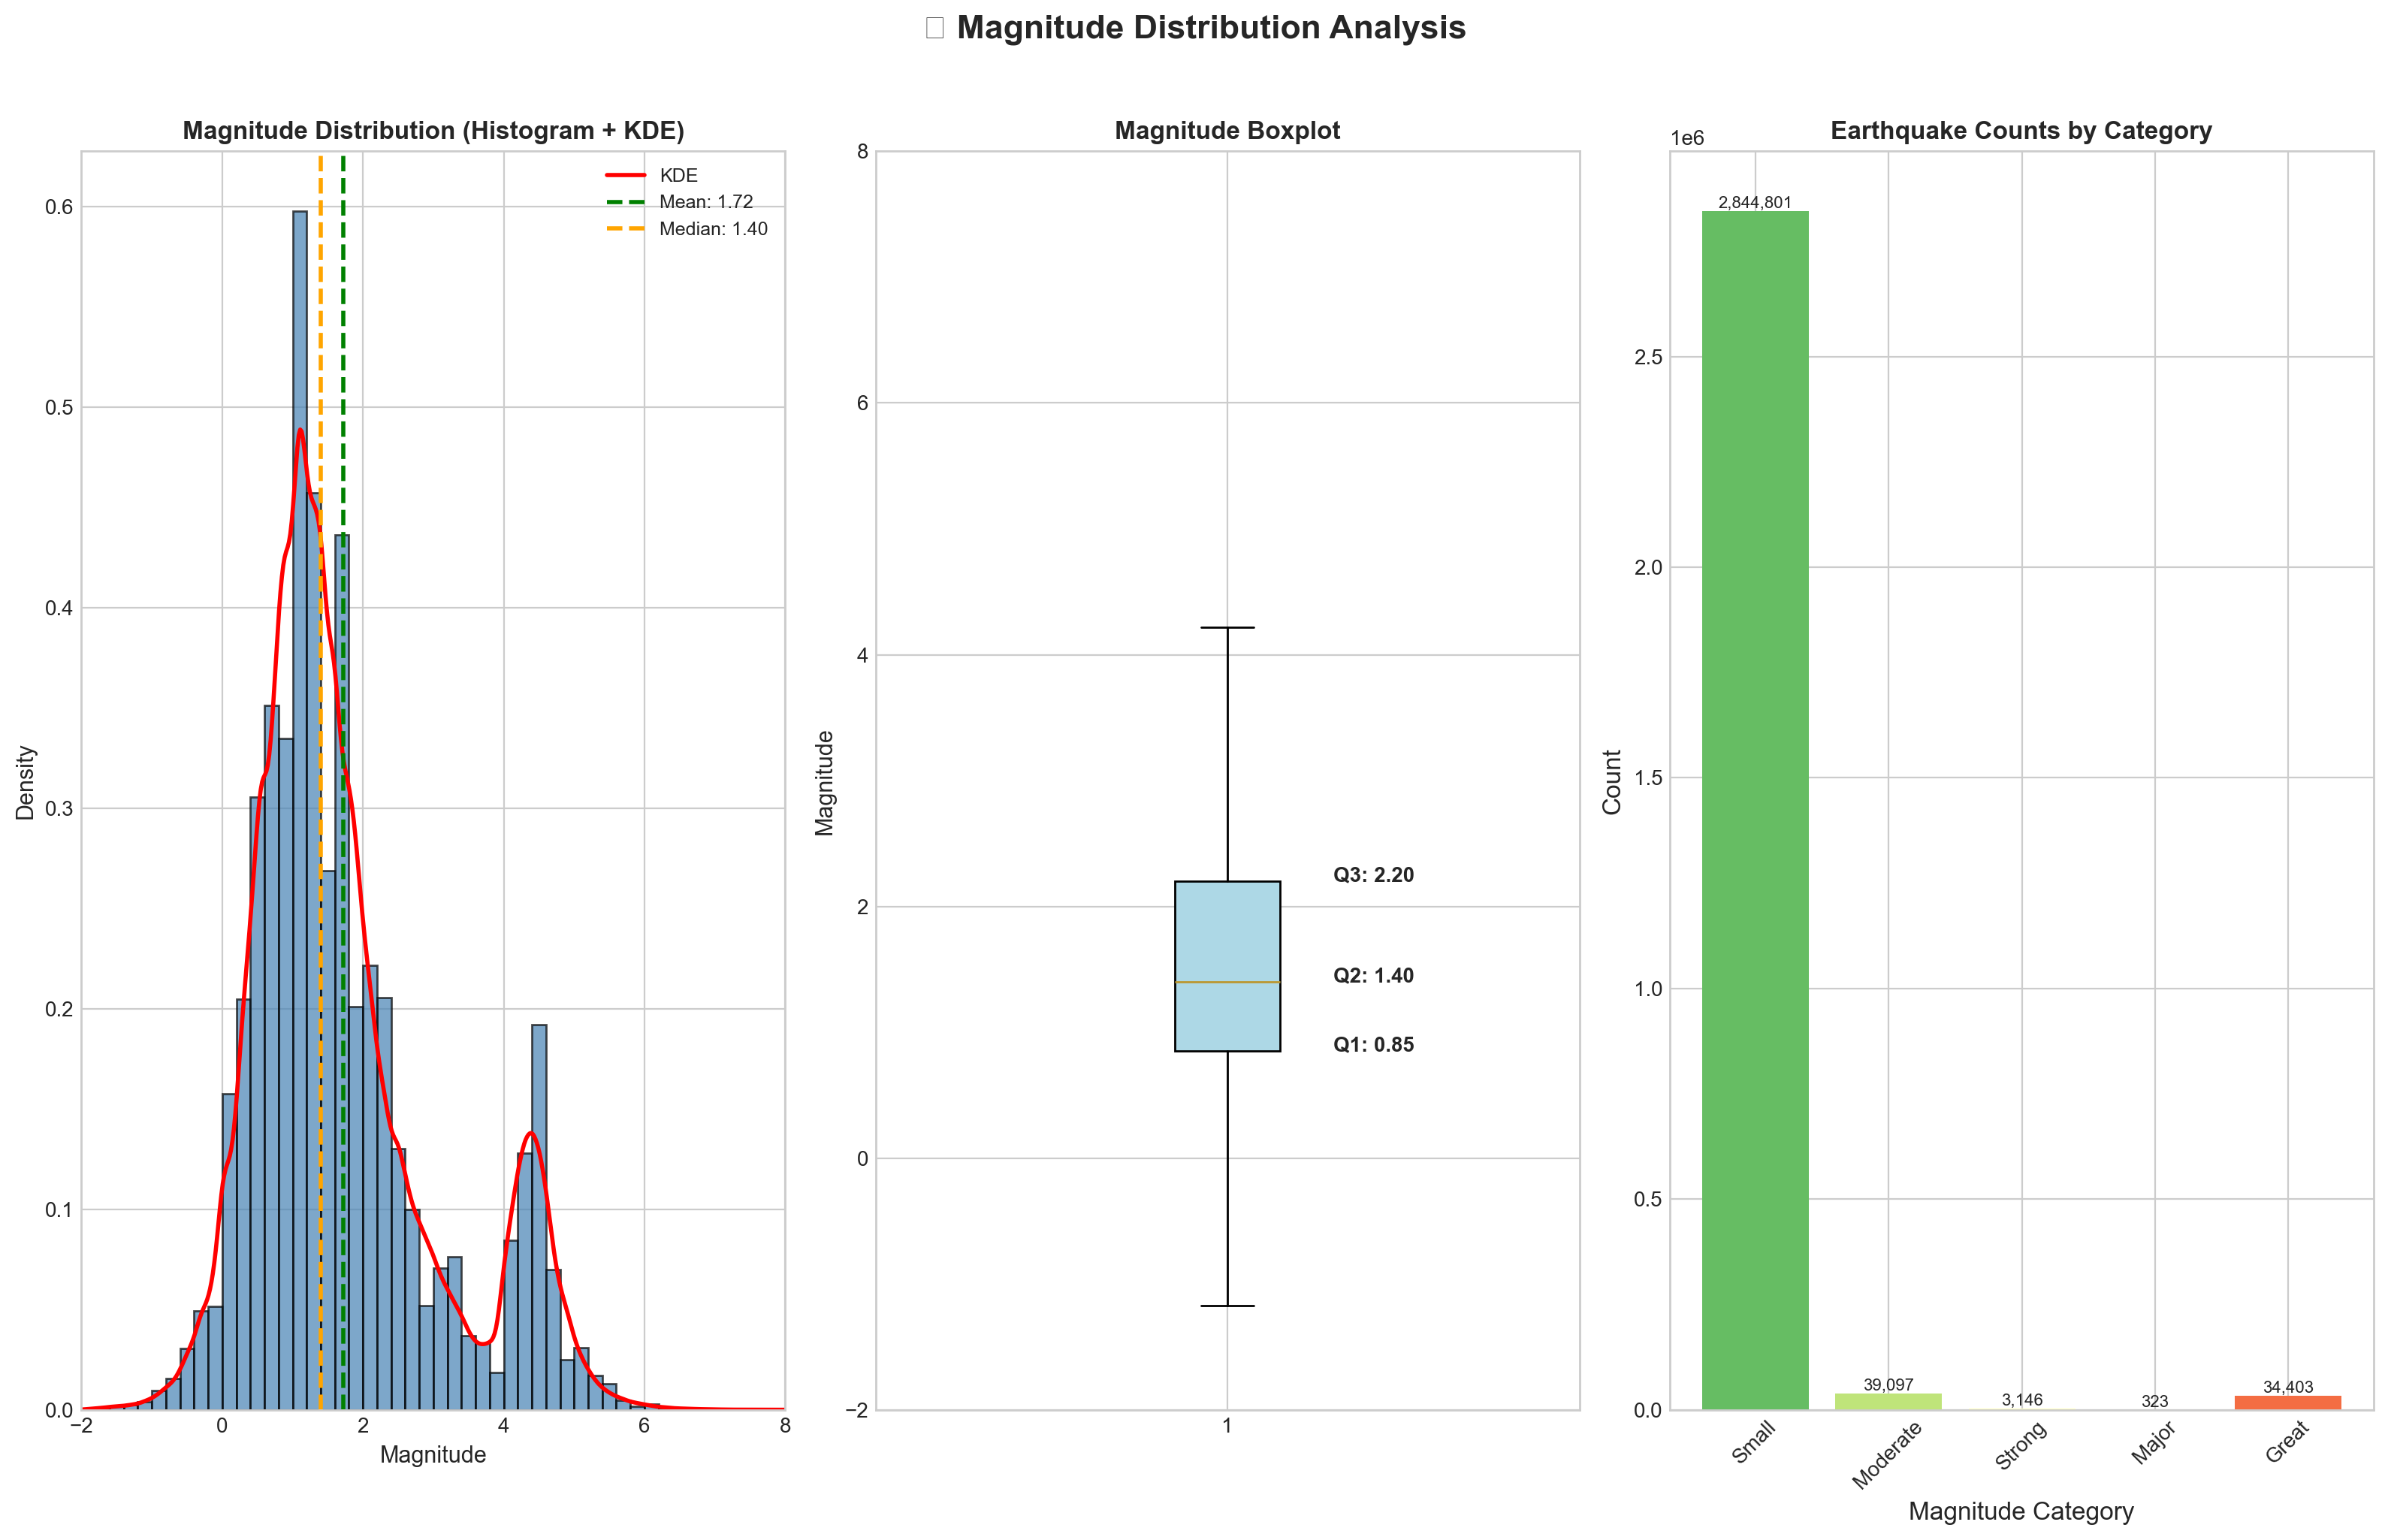
\includegraphics[width=0.95\textwidth]{figures/magnitude_distribution.png}
    \caption{Magnitude distribution analysis. Left: Histogram showing right-skewed distribution with mean=1.72 and median=1.40. Center: Boxplot with quartiles Q1=0.90, Q2=1.40, Q3=2.30. Right: Counts by magnitude category showing extreme class imbalance.}
    \label{fig:magnitude_dist}
\end{figure}

\textbf{Key statistics:}
\begin{itemize}
    \item \textbf{Mean}: 1.72, \textbf{Median}: 1.40, \textbf{Std}: 1.32
    \item \textbf{Range}: -9.99 to 9.1
    \item \textbf{Distribution}: Right-skewed (skewness = 0.85), following the Gutenberg-Richter law
\end{itemize}

\textbf{Category breakdown:}
\begin{itemize}
    \item Small (M $<$ 4.0): 2,844,801 events (\textbf{97.4\%})
    \item Moderate (4.0--5.0): 39,097 events (1.3\%)
    \item Strong (5.0--6.0): 34,403 events (1.2\%)
    \item Major (M $\geq$ 7.0): 323 events (0.01\%)
\end{itemize}

The extreme class imbalance (97.4\% small earthquakes) reflects the physics of earthquake generation---small ruptures are far more common than large ones.

\subsubsection{Depth-Magnitude Relationship}

Figure \ref{fig:depth_vs_mag} examines the relationship between earthquake depth and magnitude.

\begin{figure}[H]
    \centering
    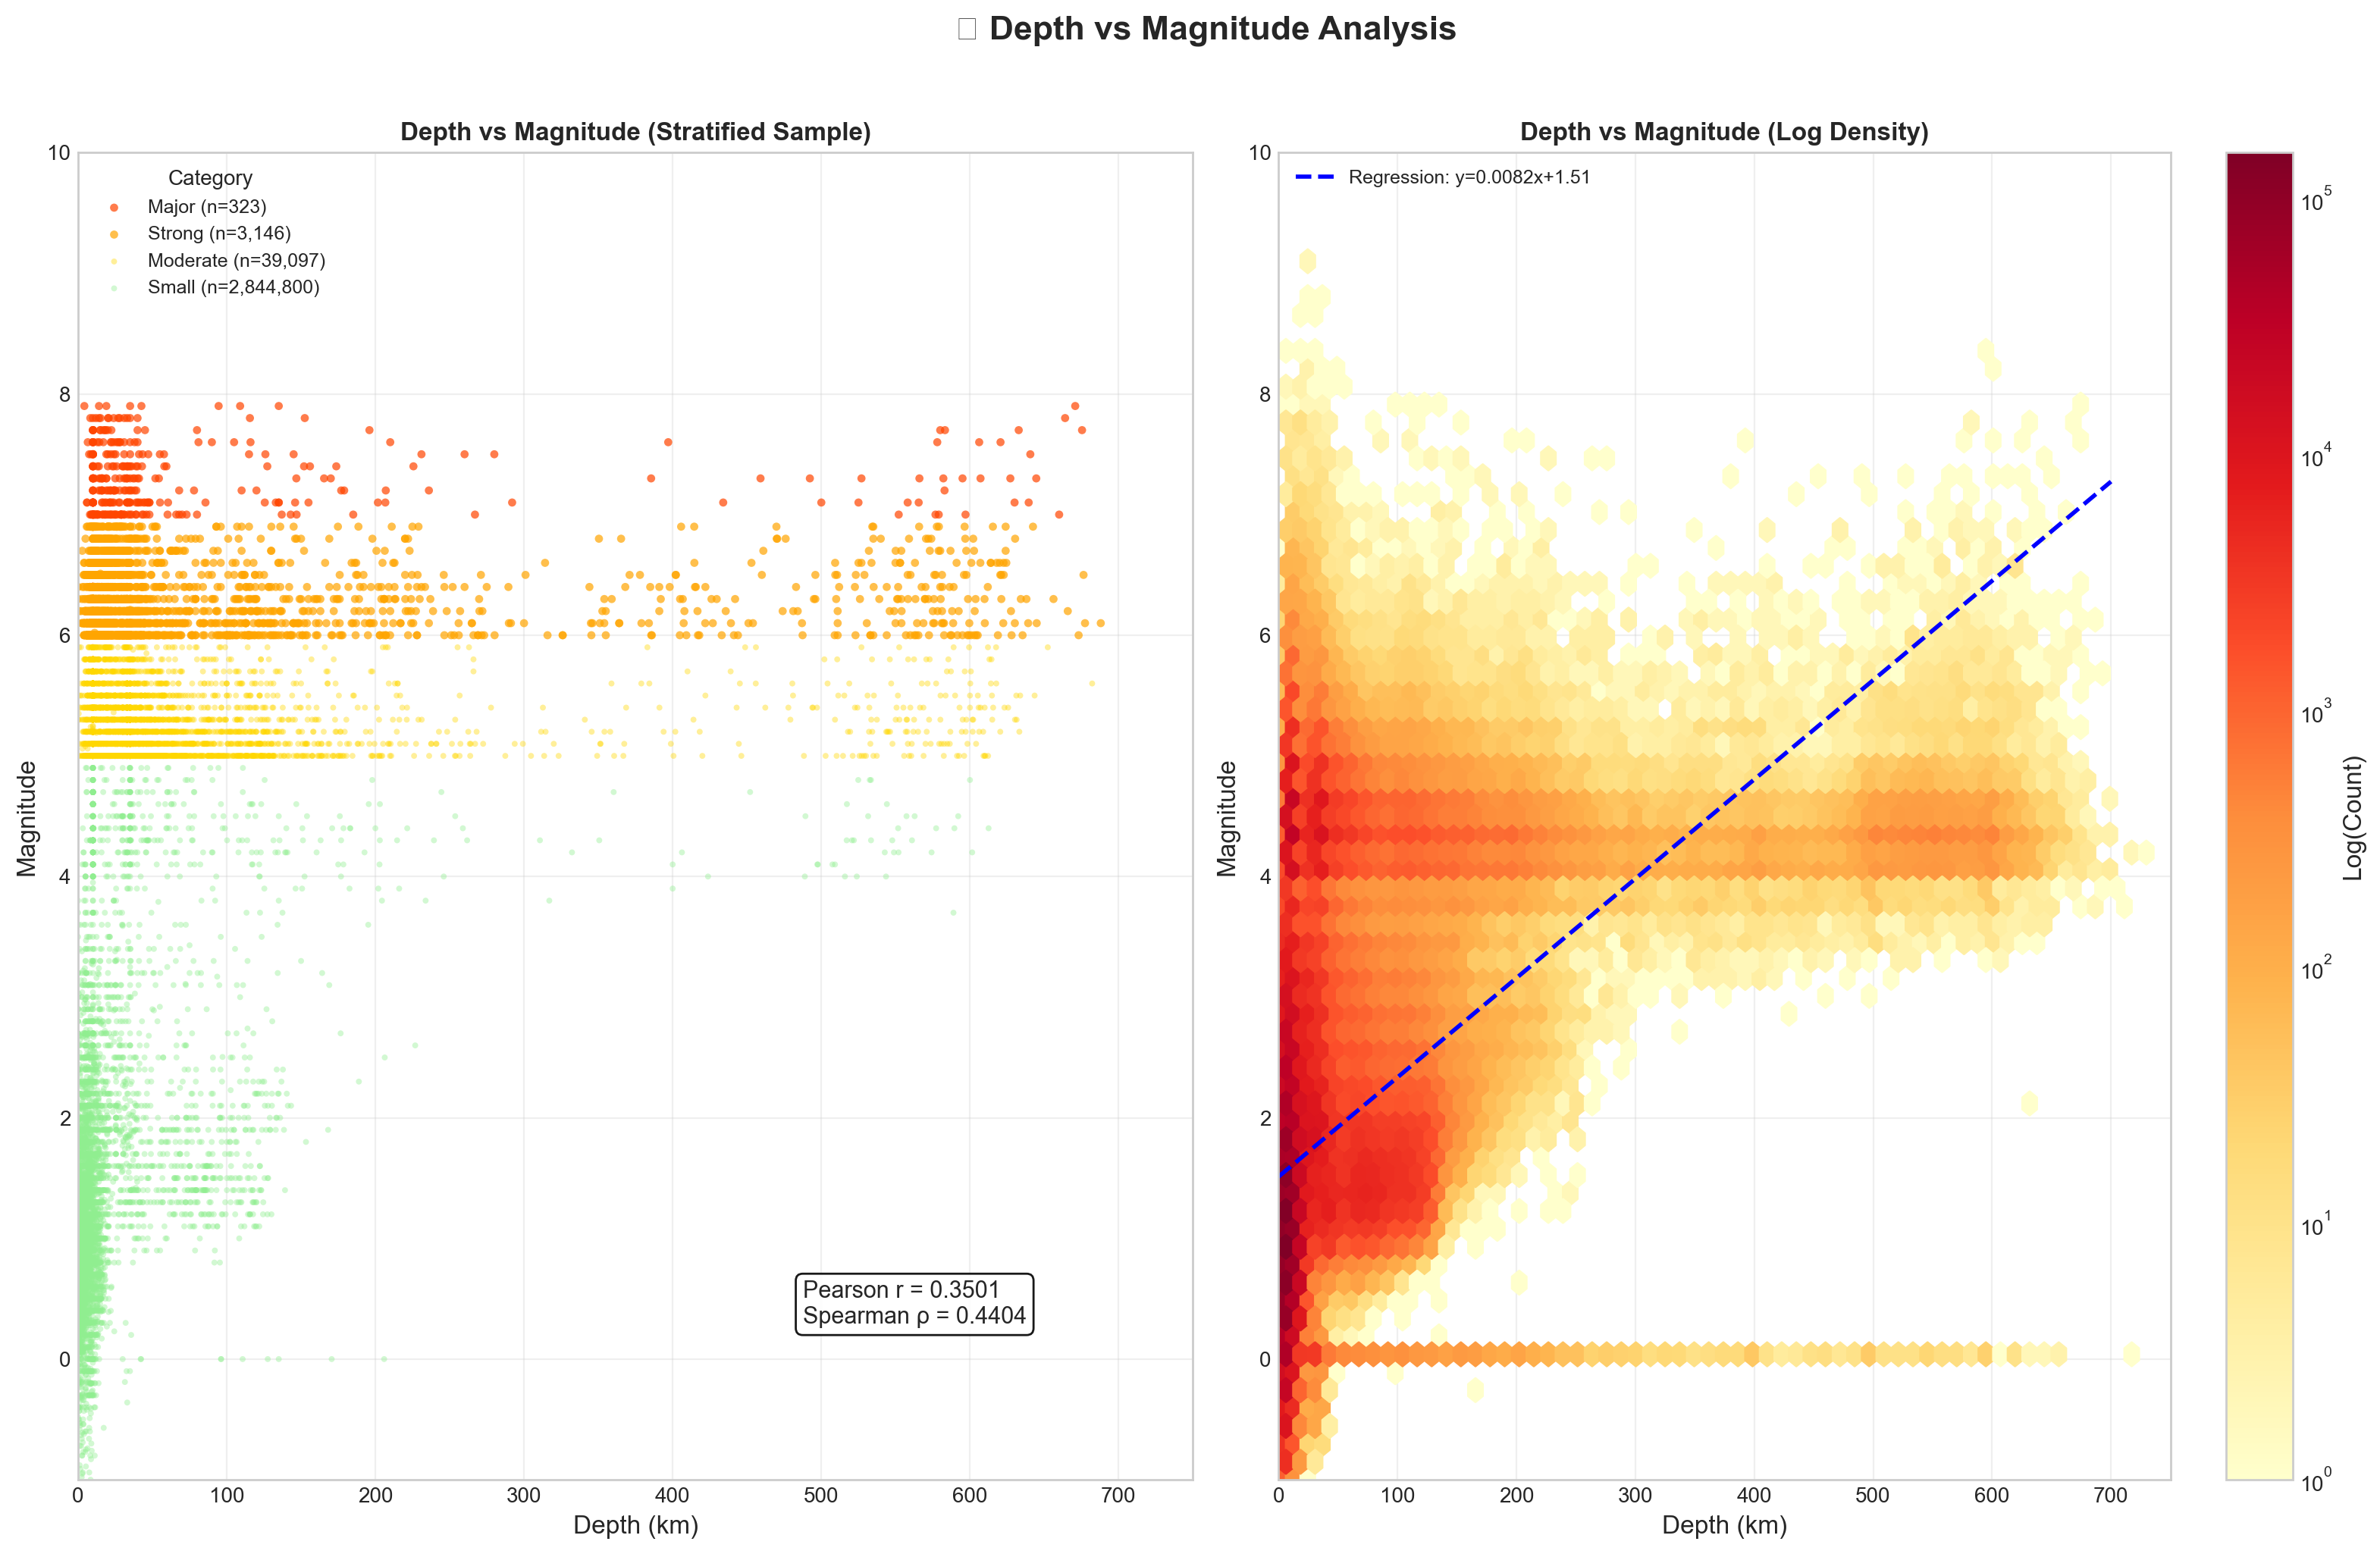
\includegraphics[width=0.95\textwidth]{figures/depth_vs_magnitude_scatter.png}
    \caption{Depth vs Magnitude relationship. Left: Stratified scatter plot showing all magnitude categories clearly with correlation statistics (Pearson r = 0.35, Spearman $\rho$ = 0.44). Right: Hexbin log-density plot showing concentration of small, shallow earthquakes with regression line.}
    \label{fig:depth_vs_mag}
\end{figure}

\textbf{Key findings:}
\begin{itemize}
    \item \textbf{Moderate positive correlation}: r = 0.35, meaning deeper earthquakes tend to have larger magnitudes on average.
    \item \textbf{Detection bias}: Small earthquakes at great depth are harder to detect---seismic waves attenuate before reaching surface seismometers.
    \item \textbf{Shallow earthquakes span all magnitudes}: From micro-earthquakes (M $<$ 0) to great earthquakes (M $>$ 8).
\end{itemize}

\subsubsection{Energy-Magnitude Relationship}

Figure \ref{fig:mag_energy} demonstrates why magnitude prediction is critical---energy scales exponentially.

\begin{figure}[H]
    \centering
    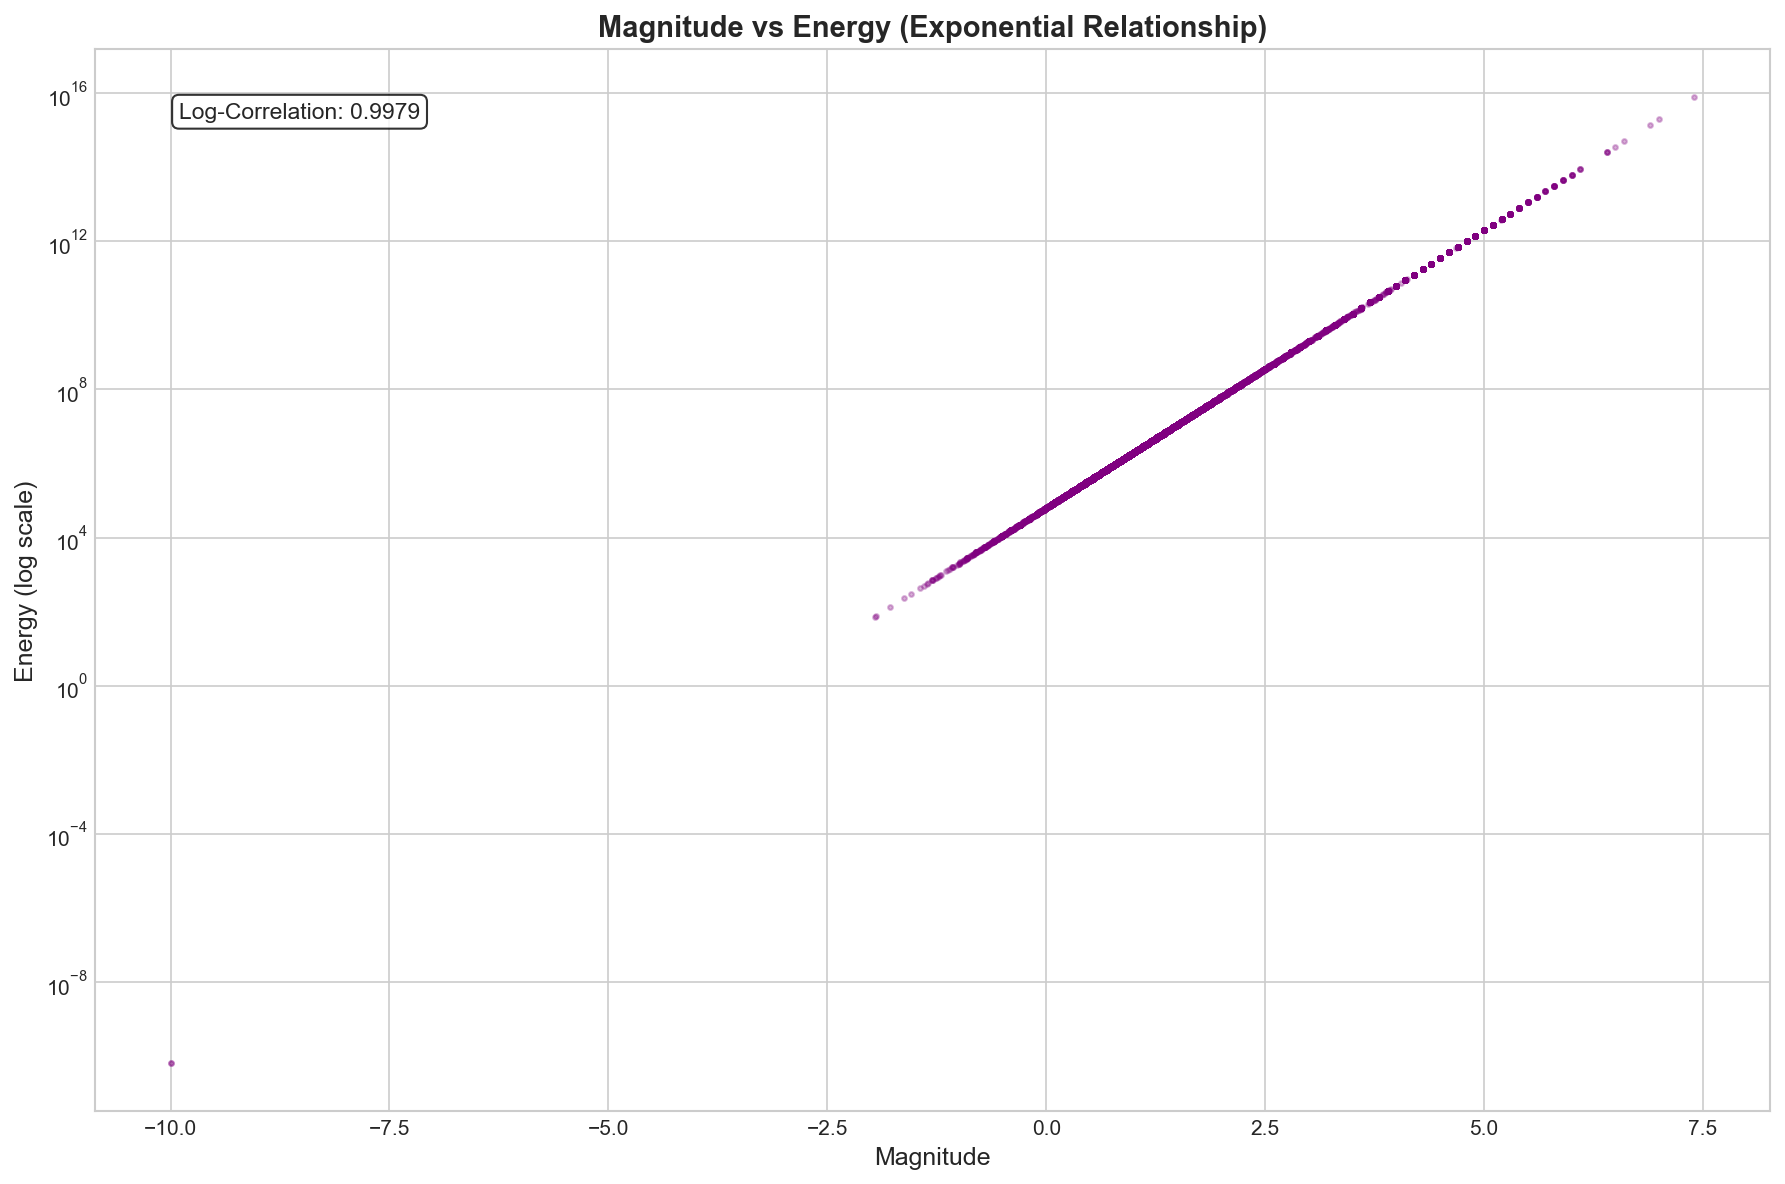
\includegraphics[width=0.75\textwidth]{figures/magnitude_vs_energy.png}
    \caption{Magnitude vs Energy on semi-log scale. Linear trend confirms exponential relationship: each magnitude unit releases approximately 31.6 times more energy.}
    \label{fig:mag_energy}
\end{figure}

The energy-magnitude relationship follows:
\begin{equation}
\log_{10}(E) = 1.5M + 4.8 \text{ (Joules)}
\end{equation}

This means a M 9.0 earthquake releases \textbf{1 million times} more energy than a M 5.0, explaining why great earthquakes cause catastrophic damage.

%==============================================================================
\subsection{Depth Analysis}
%==============================================================================

\subsubsection{Depth Distribution}

Figure \ref{fig:depth_dist} shows the distribution of earthquake depths, revealing the vertical structure of seismic activity.

\begin{figure}[H]
    \centering
    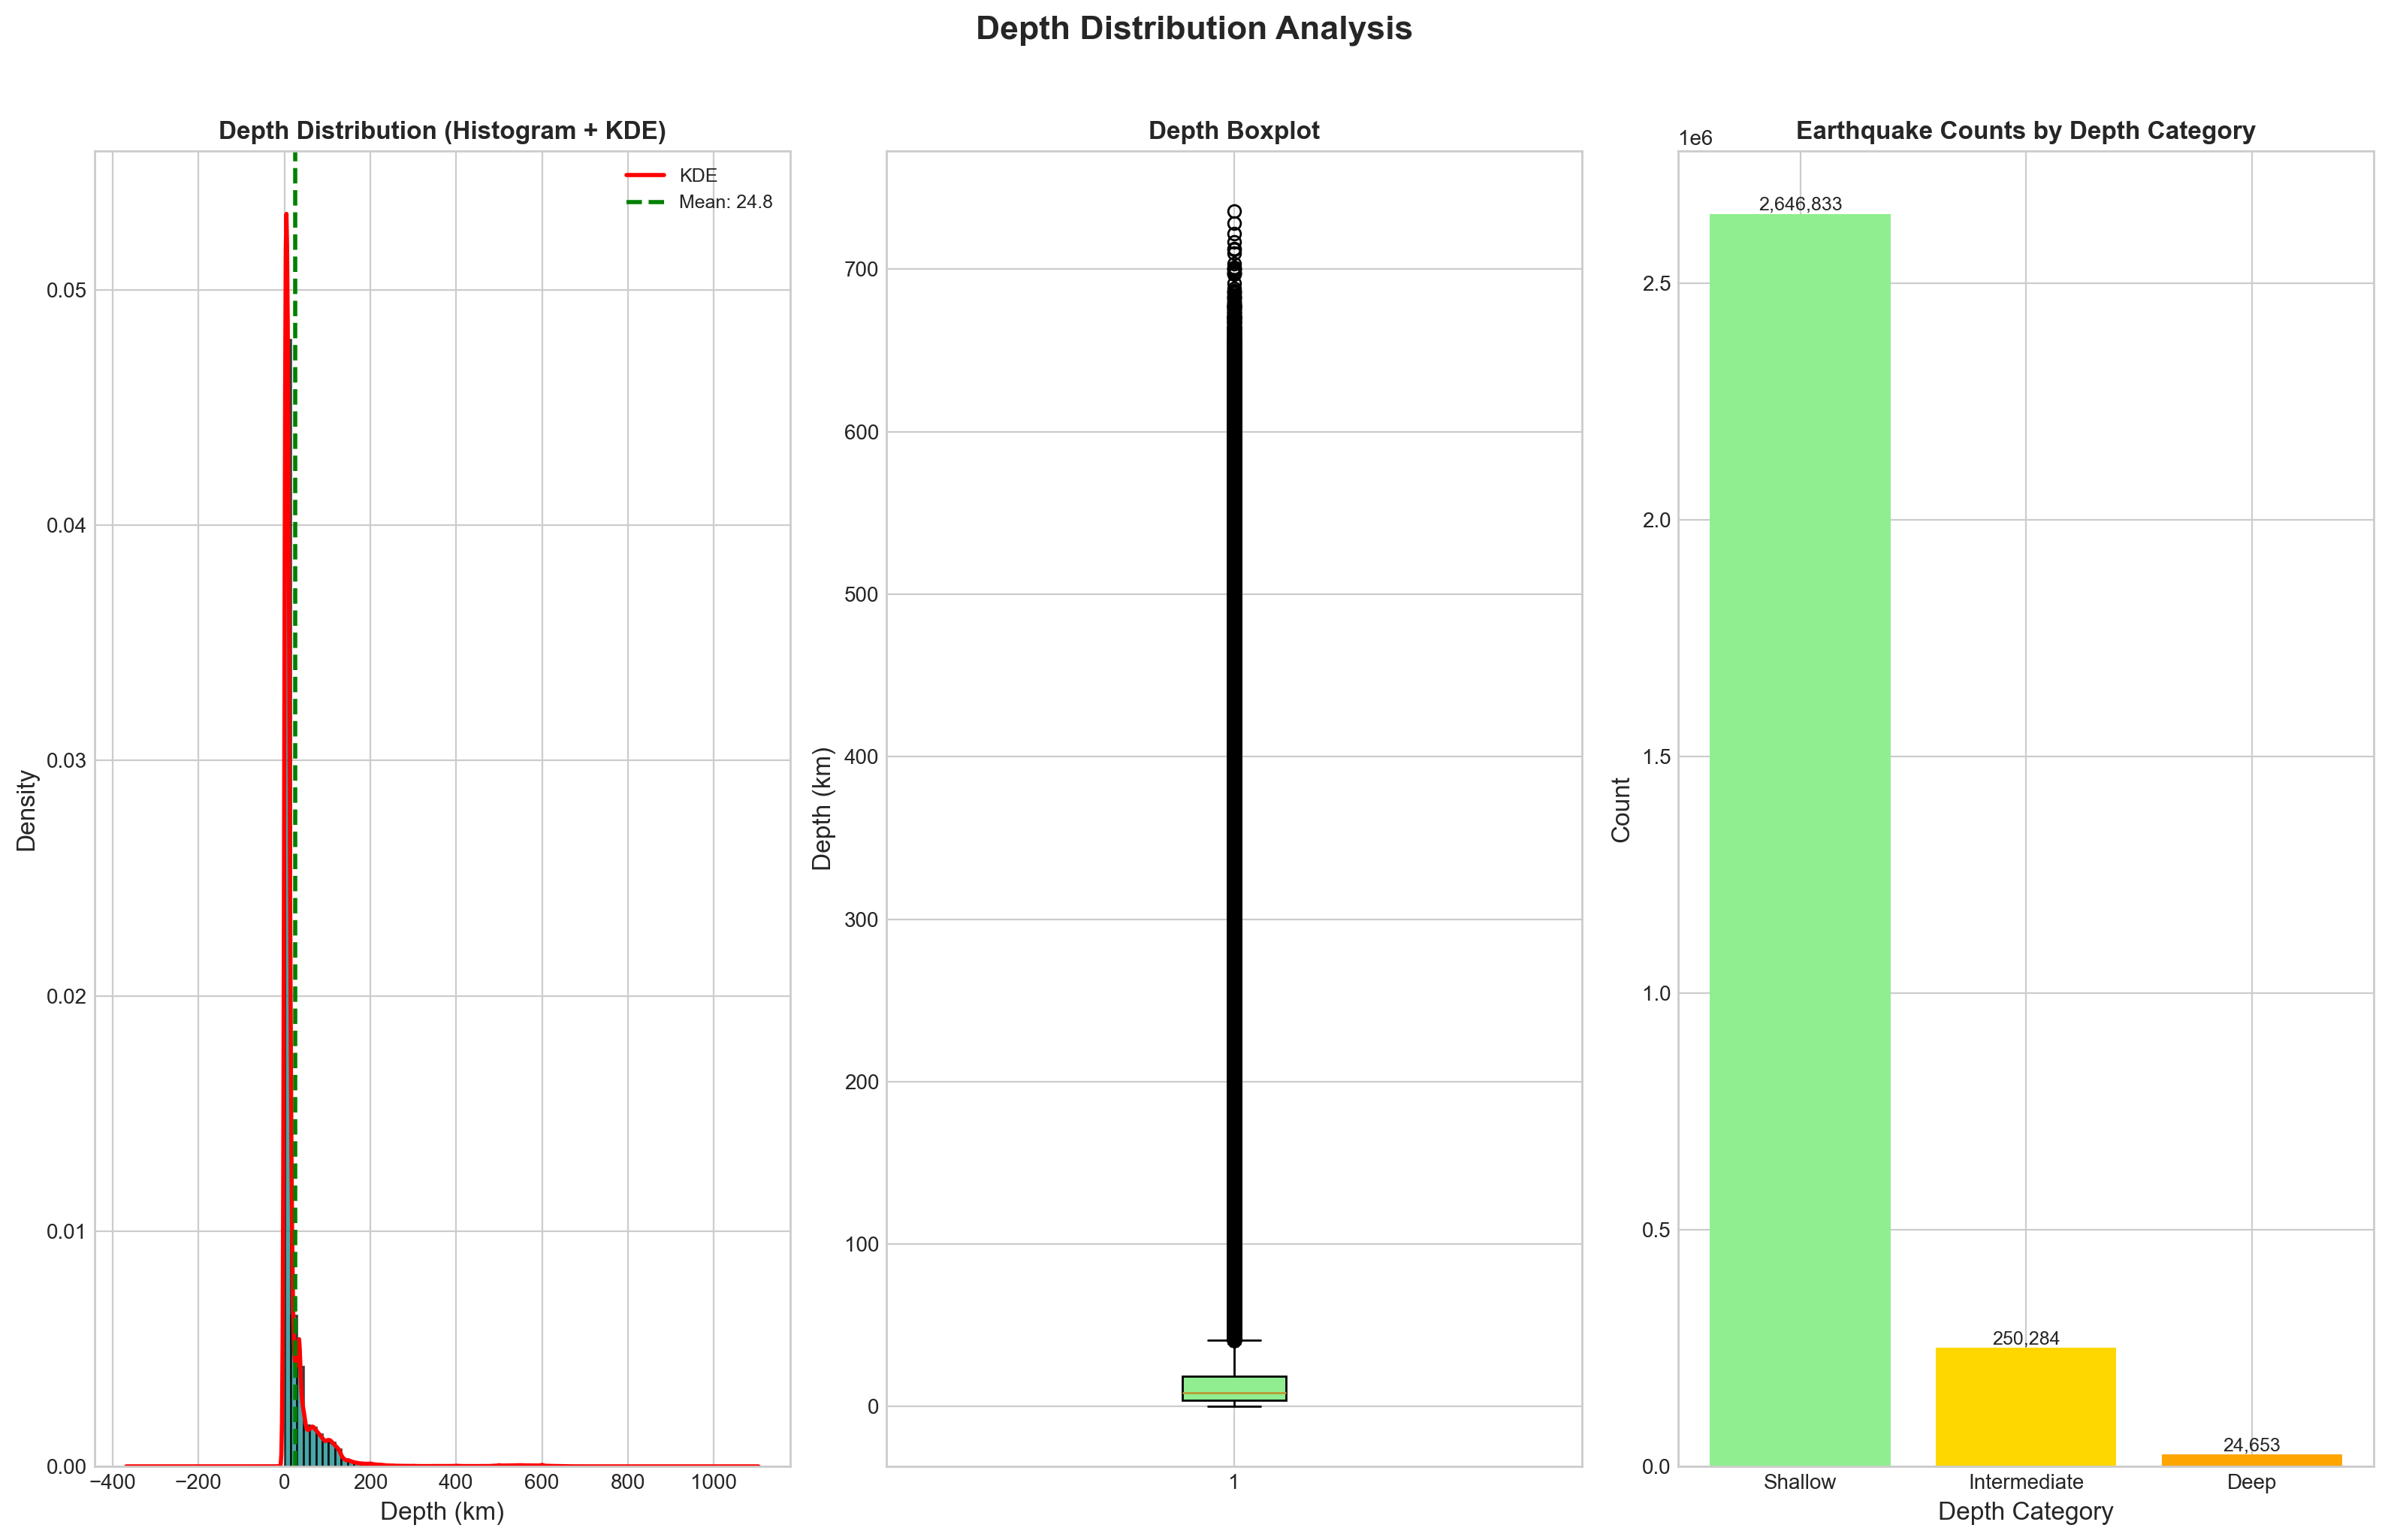
\includegraphics[width=0.95\textwidth]{figures/depth_distribution.png}
    \caption{Depth distribution analysis. Left: Histogram showing concentration at shallow depths (mean=24.8 km, median=8.6 km). Center: Boxplot showing outliers up to 735.8 km. Right: Category breakdown showing Shallow earthquakes dominate at 90.6\%.}
    \label{fig:depth_dist}
\end{figure}

\textbf{Depth statistics:}
\begin{itemize}
    \item \textbf{Mean}: 24.8 km, \textbf{Median}: 8.6 km
    \item \textbf{Maximum}: 735.8 km (near the physical limit for earthquakes)
\end{itemize}

\textbf{Category distribution:}
\begin{itemize}
    \item \textbf{Shallow} ($<$ 70 km): 2,646,833 events (\textbf{90.6\%}) --- Most destructive due to proximity to surface
    \item \textbf{Intermediate} (70--300 km): 231,458 events (7.9\%) --- Associated with subduction zones
    \item \textbf{Deep} ($>$ 300 km): 43,477 events (1.5\%) --- Only in active subduction zones (Tonga-Kermadec, South America)
\end{itemize}

\subsubsection{Geographic Patterns of Depth}

Deep earthquakes occur only in specific tectonic settings:
\begin{itemize}
    \item \textbf{Shallow earthquakes}: Occur everywhere with tectonic activity
    \item \textbf{Intermediate depth}: Concentrated in subduction zones (Japan, South America, Indonesia)
    \item \textbf{Deep earthquakes}: Only where cold oceanic lithosphere descends into the mantle
\end{itemize}

This geographic constraint means \textbf{latitude and longitude are informative features} for depth classification---certain regions simply do not produce deep earthquakes.

%==============================================================================
\subsection{Geospatial Analysis}
%==============================================================================

\subsubsection{Global Earthquake Distribution}

Figure \ref{fig:locations} shows the spatial distribution of earthquakes, revealing natural clustering patterns along tectonic plate boundaries.

\begin{figure}[H]
    \centering
    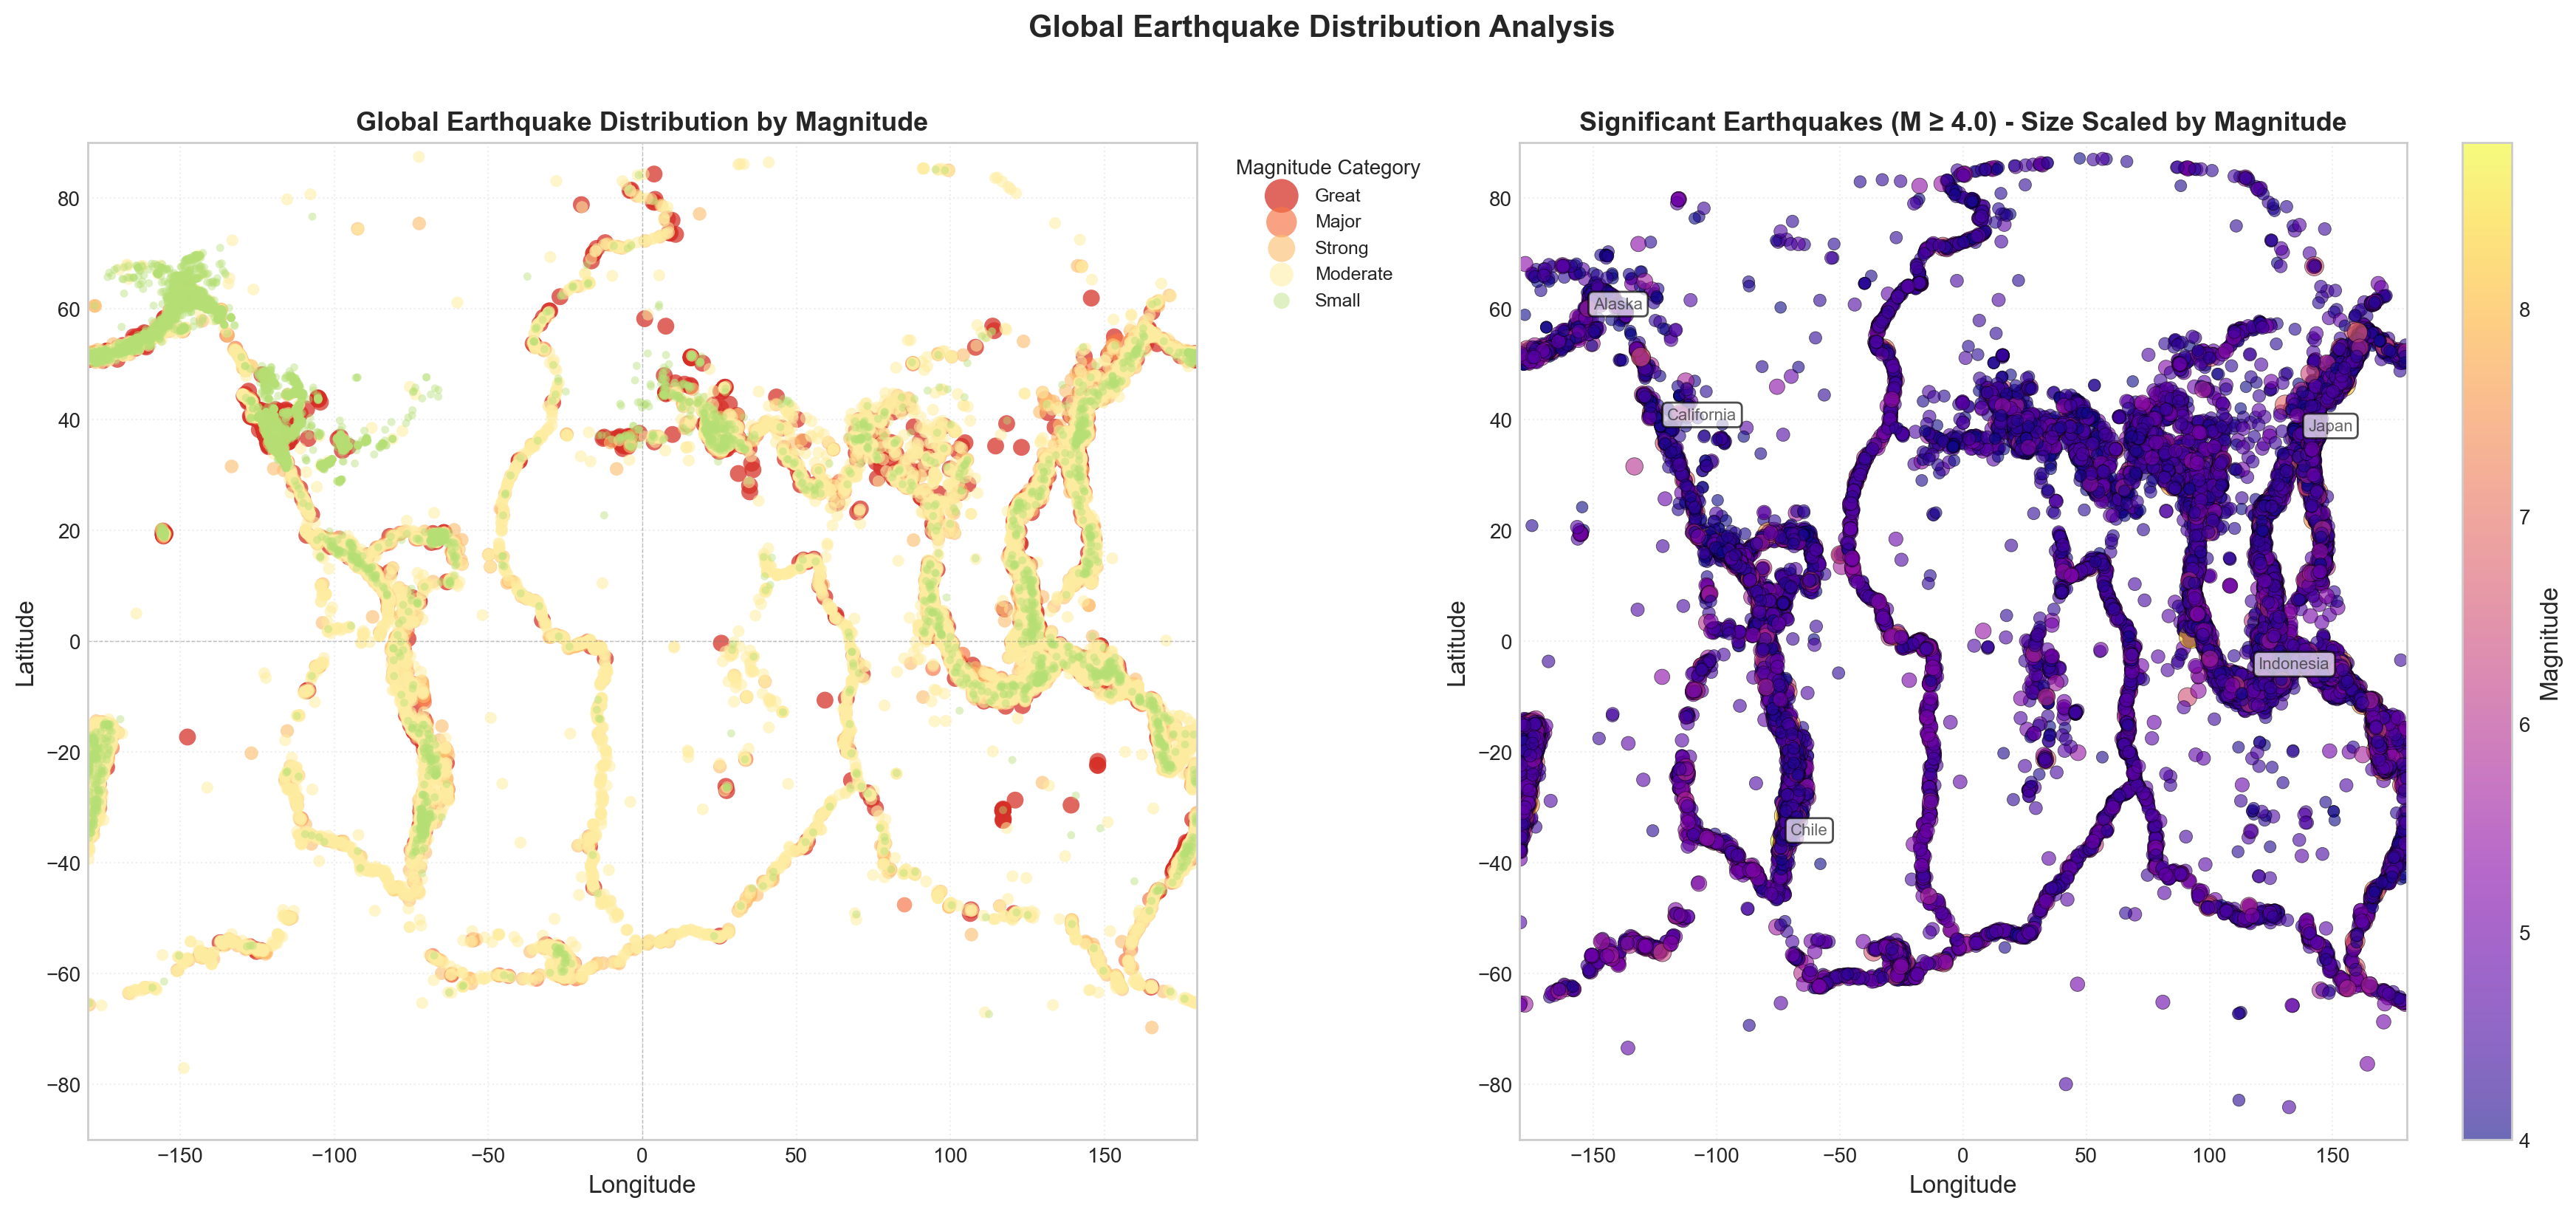
\includegraphics[width=0.95\textwidth]{figures/earthquake_locations.png}
    \caption{Global earthquake distribution. Left: All earthquakes colored by magnitude category showing concentration along plate boundaries. Right: Significant earthquakes (M $\geq$ 4.0) with annotated seismic zones. The Pacific Ring of Fire is clearly visible.}
    \label{fig:locations}
\end{figure}

\textbf{Major seismic zones identified:}
\begin{itemize}
    \item \textbf{Pacific Ring of Fire}: Accounts for $\sim$80\% of significant earthquakes, encircling the Pacific Ocean
    \item \textbf{California/San Andreas}: Dense cluster along transform fault
    \item \textbf{Alaska-Aleutian}: High-frequency cluster at subduction zone
    \item \textbf{Japan-Kamchatka}: Major subduction zone cluster
    \item \textbf{Indonesia}: Sunda arc subduction cluster
    \item \textbf{Chile/South America}: Nazca plate subduction cluster
\end{itemize}

\subsubsection{Earthquake Density Heatmap}

Figure \ref{fig:density} provides density visualization essential for identifying seismic hotspots.

\begin{figure}[H]
    \centering
    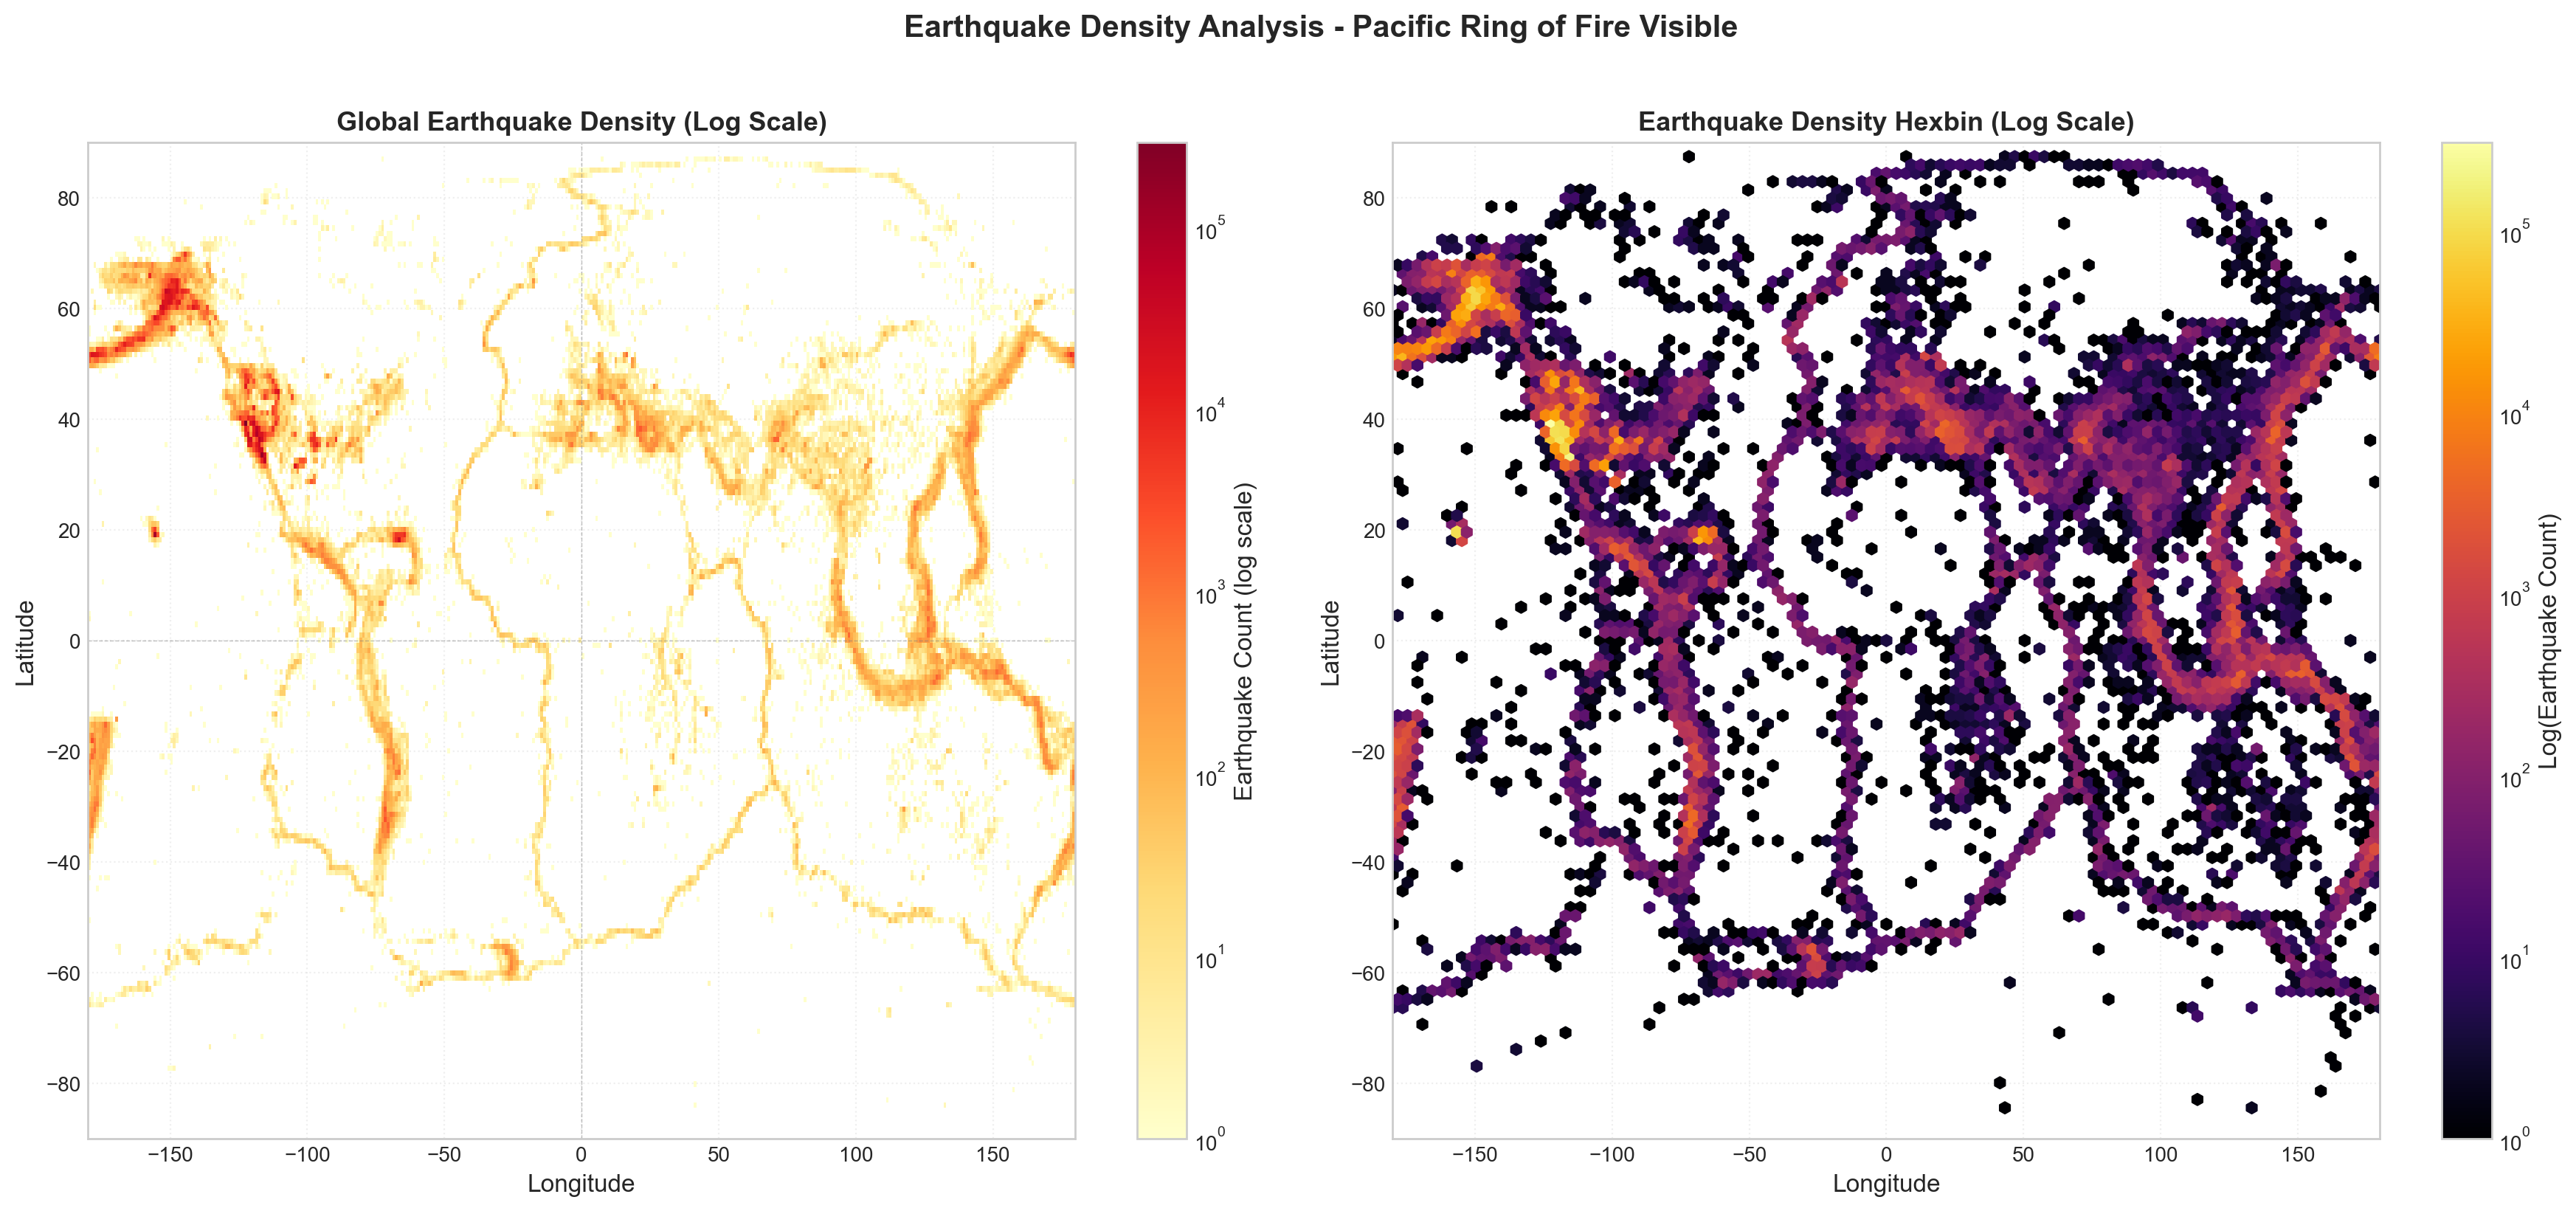
\includegraphics[width=0.95\textwidth]{figures/earthquake_density.png}
    \caption{Earthquake density heatmap with logarithmic color scale. Left: 2D histogram (1-degree resolution). Right: Hexbin smoothed visualization. High-density regions represent seismic hotspots along plate boundaries.}
    \label{fig:density}
\end{figure}

The density map validates tectonic theory---seismicity follows plate boundaries with remarkable precision. The Pacific Ring of Fire clearly emerges as the dominant seismic belt.

\subsubsection{Regional Statistics}

Figure \ref{fig:regional} quantifies earthquake frequency and intensity by region.

\begin{figure}[H]
    \centering
    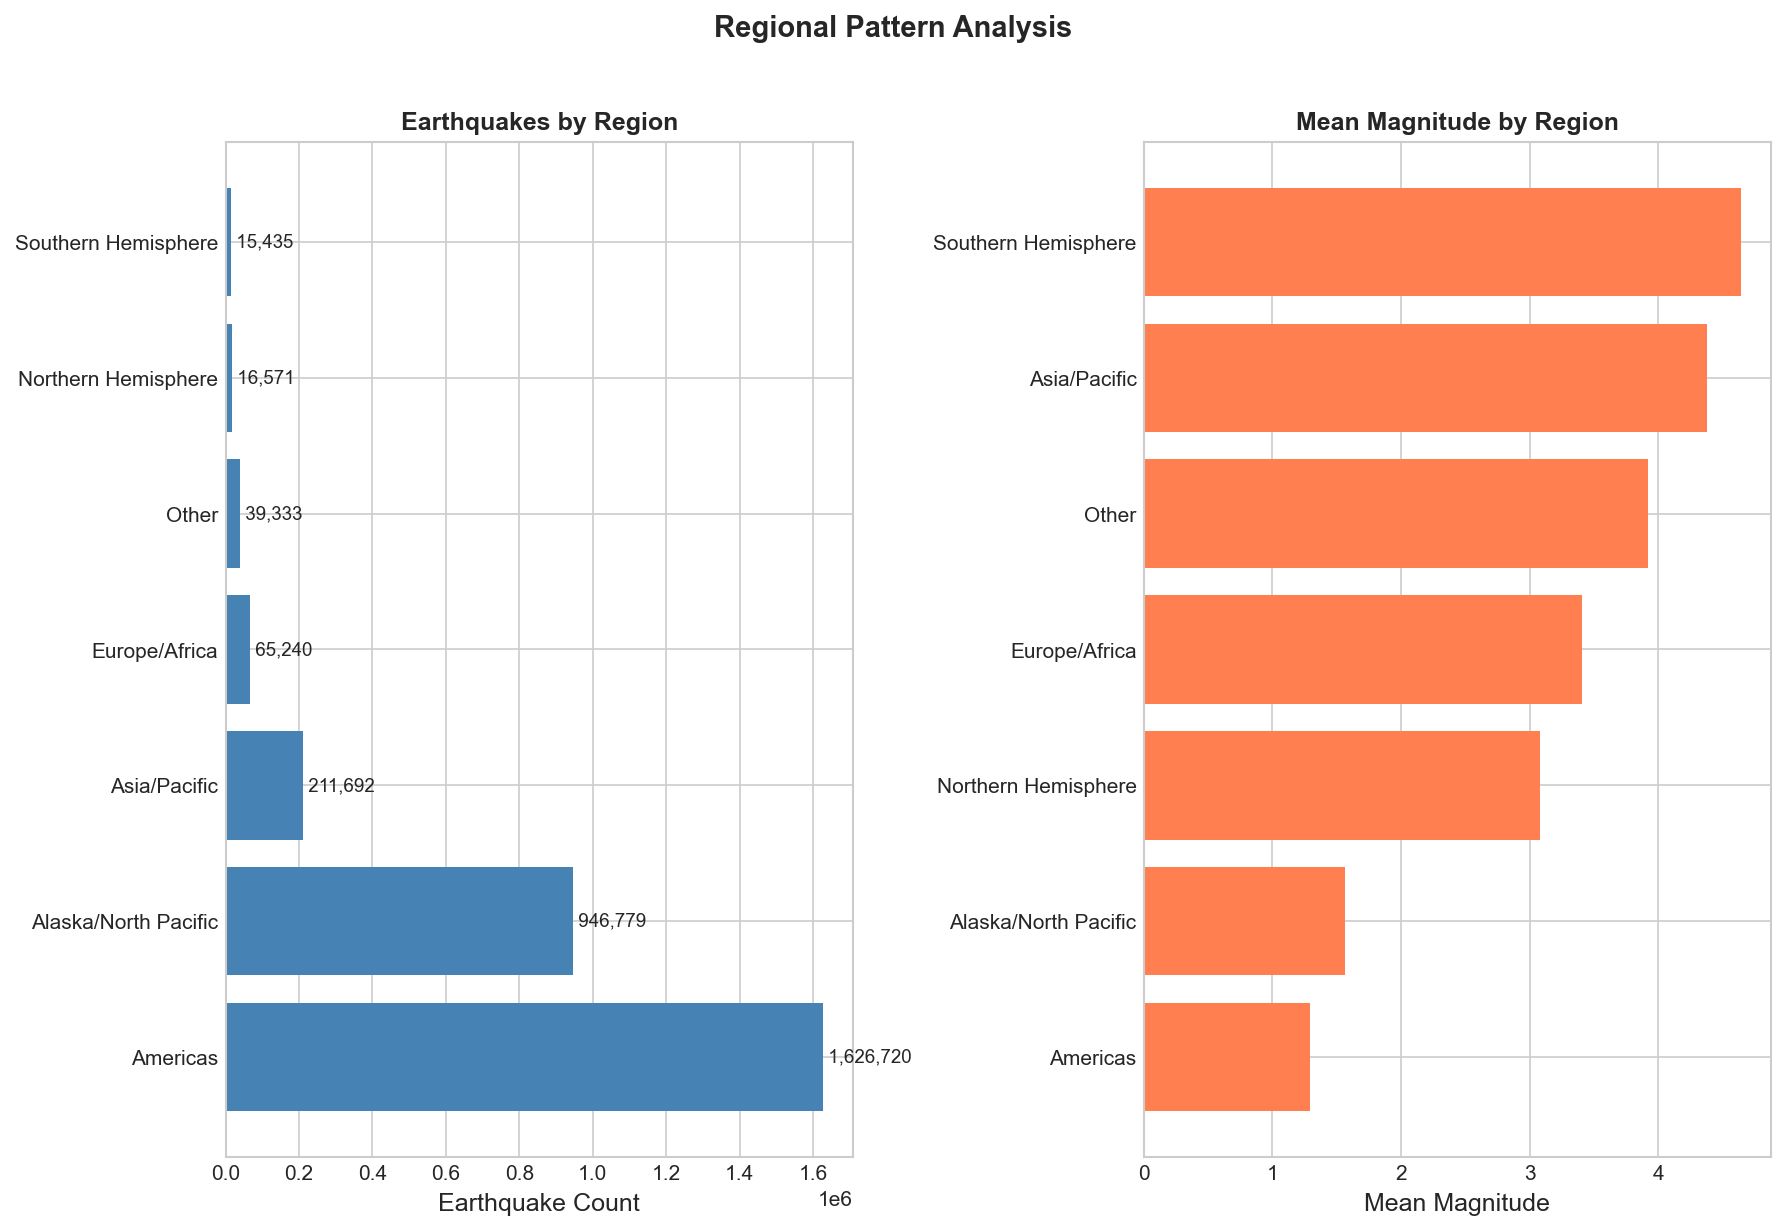
\includegraphics[width=0.85\textwidth]{figures/regional_patterns.png}
    \caption{Regional earthquake patterns. Left: Event counts showing Americas with highest count (1.6M events). Right: Mean magnitude by region showing Asia/Pacific with highest average (4.38).}
    \label{fig:regional}
\end{figure}

\textbf{Regional findings:}
\begin{itemize}
    \item \textbf{Americas}: 1,595,101 events, mean magnitude 1.47 --- Highest count due to dense monitoring
    \item \textbf{Alaska/North Pacific}: 946,527 events, mean magnitude 1.85
    \item \textbf{Asia/Pacific}: 210,166 events, mean magnitude \textbf{4.38} --- Fewer events but much larger on average
    \item \textbf{Detection bias}: Regions with dense networks detect more small earthquakes; less-monitored regions only record larger events
\end{itemize}

%==============================================================================
\subsection{Temporal Trends}
%==============================================================================

Figure \ref{fig:temporal} examines earthquake patterns over time.

\begin{figure}[H]
    \centering
    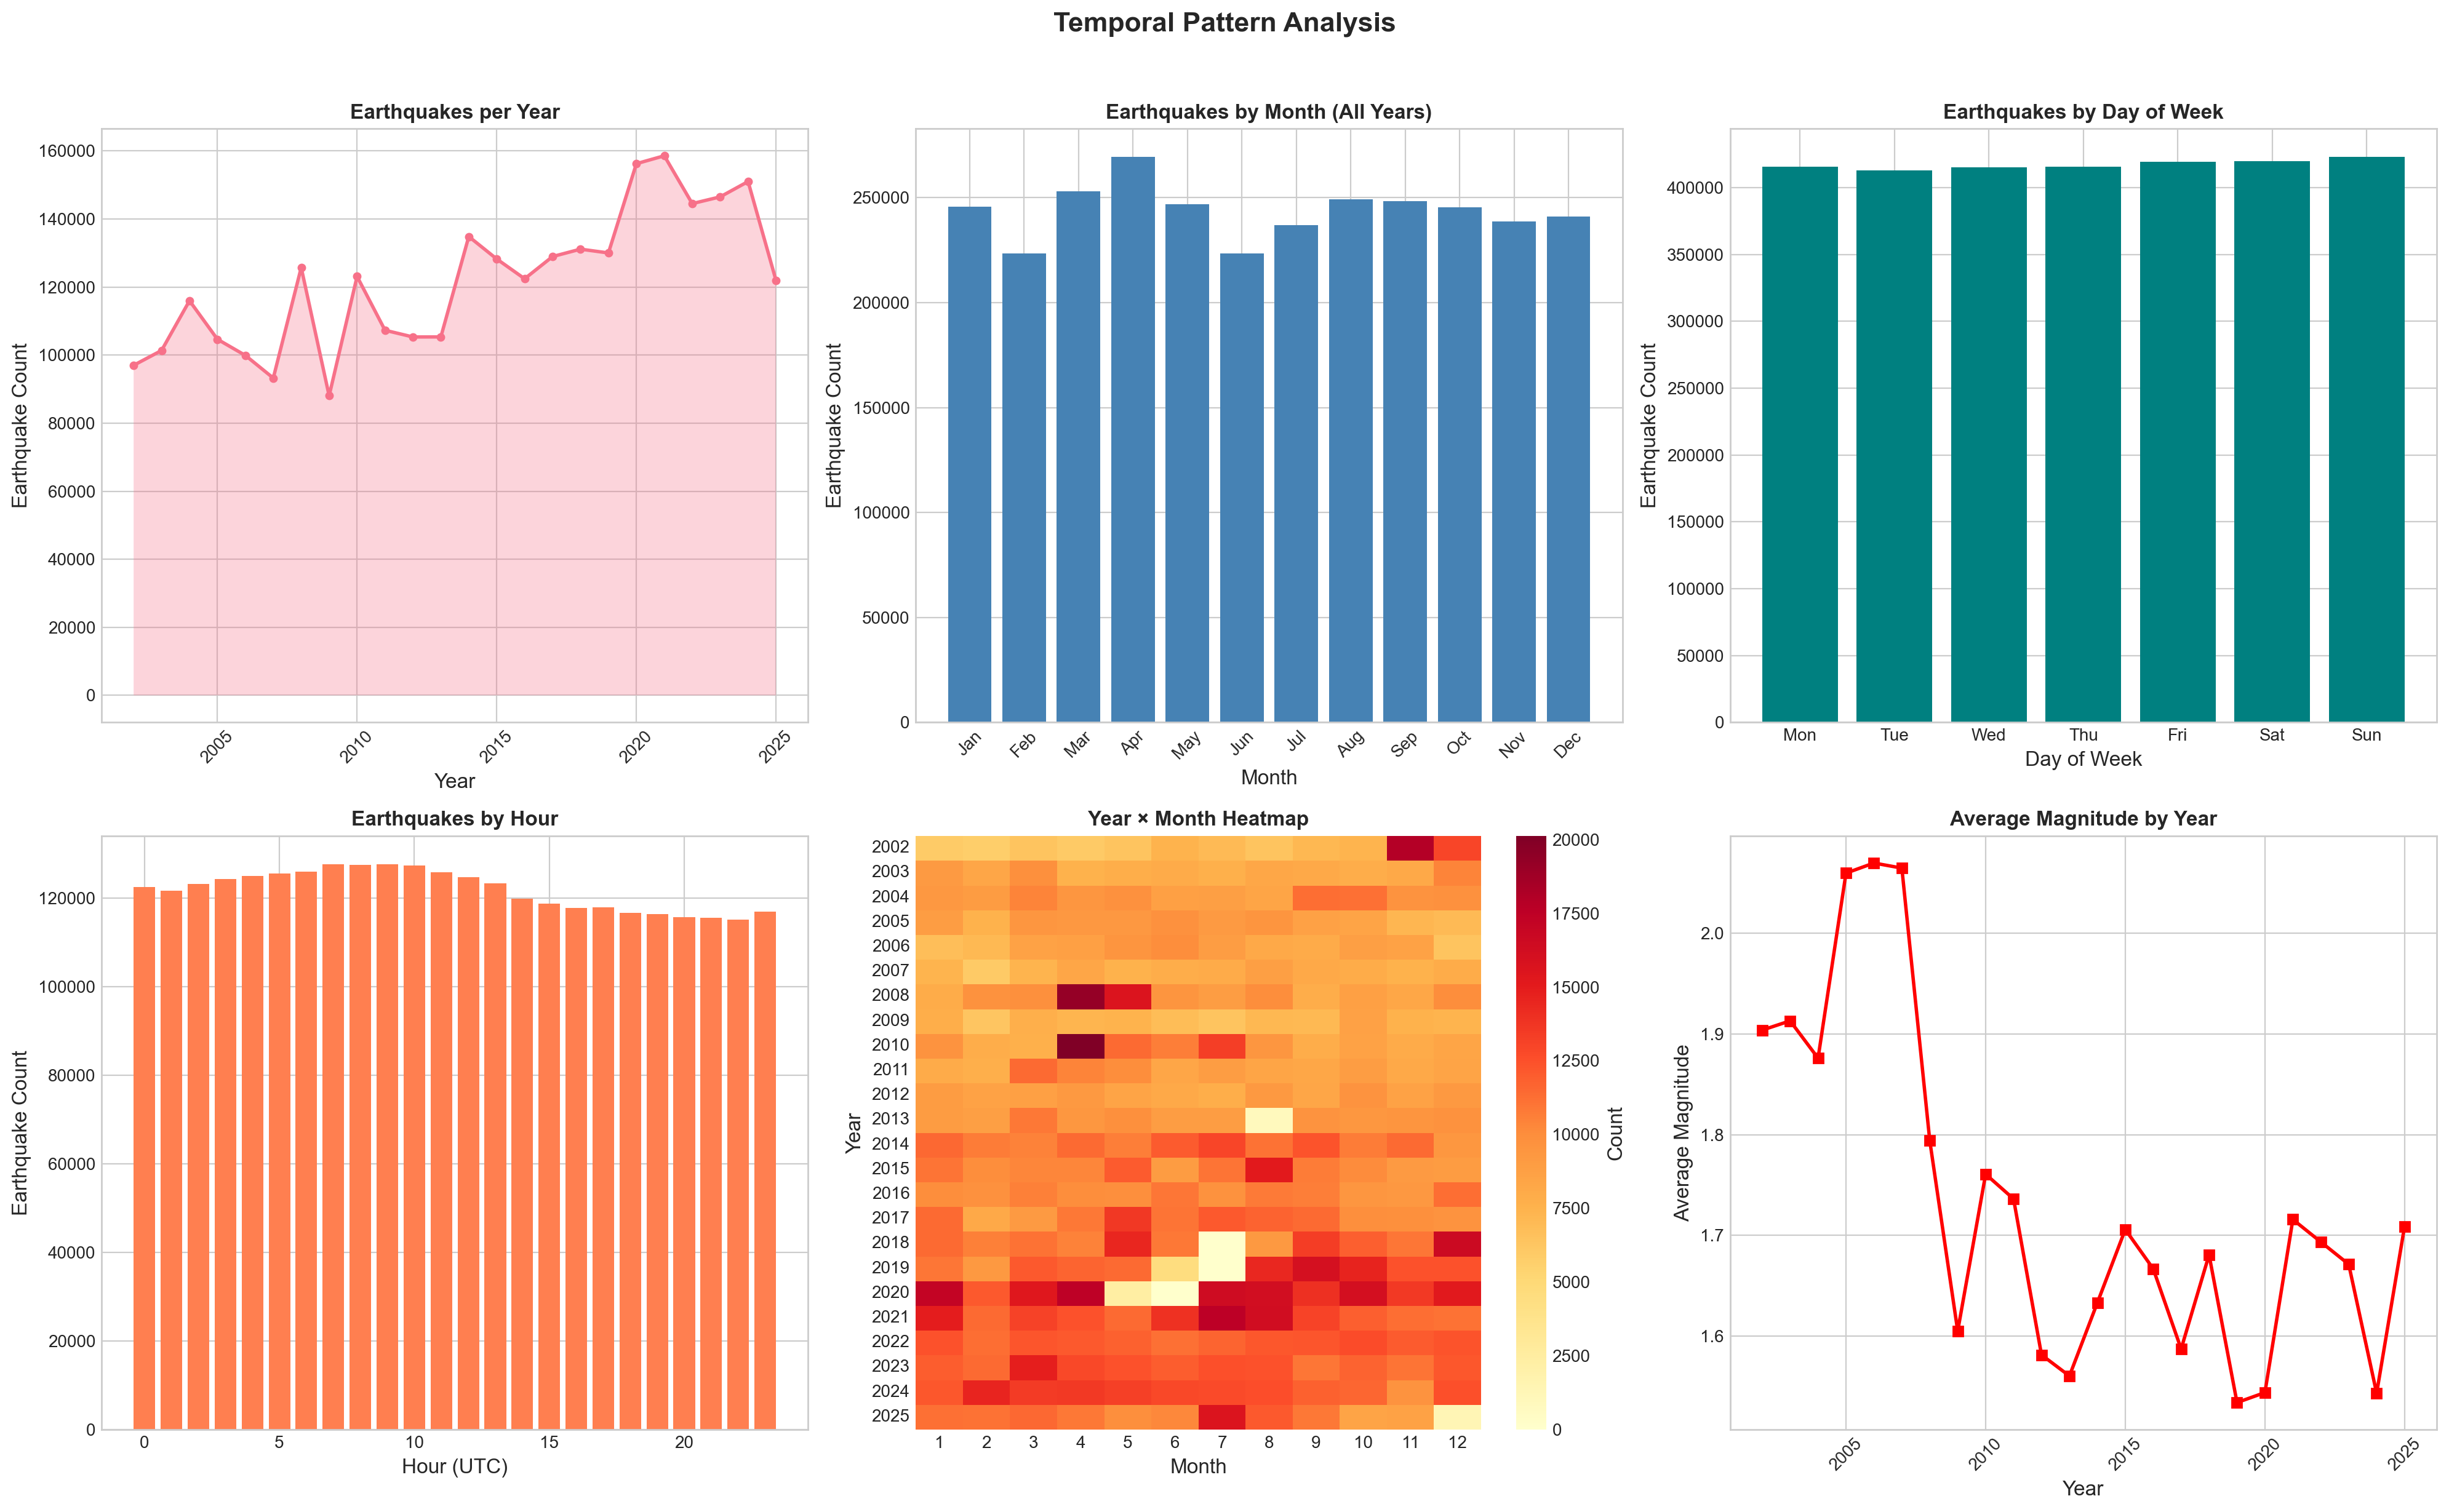
\includegraphics[width=0.95\textwidth]{figures/temporal_patterns.png}
    \caption{Temporal pattern analysis. Top-left: Yearly counts showing apparent increase from 2002--2025. Bottom-right: Average magnitude remaining stable around 1.7.}
    \label{fig:temporal}
\end{figure}

\textbf{Key insight}: The apparent increase in earthquake counts over time does \textbf{not} indicate more earthquakes are occurring. Evidence:
\begin{itemize}
    \item Average magnitude has remained stable around 1.7
    \item The increase is entirely in small earthquakes
    \item Cause: Expansion of seismic monitoring networks and improved detection
\end{itemize}

%==============================================================================
\subsection{Key Findings Summary}
%==============================================================================

\begin{table}[H]
\centering
\begin{tabular}{|p{4cm}|p{9cm}|}
\hline
\textbf{Finding} & \textbf{Implication} \\
\hline
97.4\% small earthquakes (M $<$ 4) & Severe class imbalance; need weighted sampling or loss functions \\
\hline
90.6\% shallow earthquakes & Depth classification heavily imbalanced toward Shallow class \\
\hline
Depth-Magnitude correlation r=0.35 & Depth is a useful predictive feature for magnitude \\
\hline
Pacific Ring of Fire = 80\% of large earthquakes & Strong spatial clustering; geographic features highly informative \\
\hline
Deep earthquakes only in subduction zones & Location (lat/lon) can predict depth category \\
\hline
Detection bias in counts & More monitoring $\rightarrow$ more small earthquakes detected \\
\hline
\end{tabular}
\caption{Summary of EDA findings and modeling implications}
\end{table}

\textbf{Data challenges to address:}
\begin{itemize}
    \item \textbf{Class imbalance}: Both magnitude and depth distributions are heavily skewed
    \item \textbf{Detection bias}: Station count (nst) correlates with magnitude but may not be causal
    \item \textbf{Geographic bias}: Dense monitoring in Americas skews toward detecting small earthquakes
\end{itemize}

\section{Feature Selection}
\input{sources/6_feature_selection}
\section{Experiment \& Result}
% Experiment & Result Section
% Earthquake Prediction Problems - Data Science Report

This section presents the experimental setup, model implementations, and results for three machine learning tasks: magnitude regression, depth category classification, and seismic hotspot clustering.

\subsection{Experimental Setup}

\subsubsection{Computing Environment}

All experiments were conducted using Python 3.10 with standard data science libraries. The primary libraries used include Pandas 2.0 for data manipulation, NumPy 1.24 for numerical computing, Scikit-learn 1.3 for machine learning algorithms, and Matplotlib 3.7 with Seaborn 0.12 for visualization. Experiments were executed on a system with 16GB RAM and an Intel Core i7 processor.

\subsubsection{Data Preparation}

The dataset was prepared following the feature selection process described in Section 6. The final dataset contains 2,886,684 records after removing instances with missing values in critical features. The data was split into training (70\%), validation (15\%), and test (15\%) sets using stratified sampling to maintain class proportions for classification tasks.

Due to the large dataset size, a stratified sample of 500,000 records was used for initial model development and hyperparameter tuning. Final models were trained on the full training set to maximize performance. All numerical features were standardized using z-score normalization with parameters computed from the training set only to prevent data leakage.

\subsection{Task 1: Magnitude Regression}

\subsubsection{Task Definition}

The objective of this task is to predict the exact magnitude value of earthquakes using regression techniques. Unlike categorical classification, regression provides continuous magnitude estimates that enable finer-grained risk assessment and early warning applications.

\subsubsection{Input Features}

The input features for magnitude regression include latitude representing the north-south epicenter position, longitude representing the east-west epicenter position, depth of the earthquake hypocenter in kilometers, azimuthal gap (gap) indicating the quality of station coverage, and number of recording stations (nst). These features were selected based on their correlation with magnitude observed during exploratory data analysis.

\subsubsection{Model Implementation}

Random Forest Regressor was implemented as the primary algorithm for this task. Random Forest is an ensemble method that combines multiple decision trees through bootstrap aggregation (bagging) to reduce variance and improve generalization. The model naturally handles nonlinear relationships and feature interactions without requiring extensive feature engineering.

The model was configured with 100 estimators (trees) in the ensemble, maximum tree depth of 20 to prevent overfitting, minimum samples per leaf of 10 for regularization, and the square root of total features considered at each split. Hyperparameters were tuned using 5-fold cross-validation on the training set.

\subsubsection{Evaluation Metrics}

Two primary metrics were used to evaluate regression performance. Root Mean Square Error (RMSE) measures the average prediction error in magnitude units, calculated as $RMSE = \sqrt{\frac{1}{n}\sum_{i=1}^{n}(y_i - \hat{y}_i)^2}$. R-squared (R2) Score measures the proportion of variance in magnitude explained by the model, calculated as $R^2 = 1 - \frac{\sum_{i=1}^{n}(y_i - \hat{y}_i)^2}{\sum_{i=1}^{n}(y_i - \bar{y})^2}$.

\subsubsection{Results}

Table \ref{tab:regression_results} presents the performance of Random Forest Regressor on the magnitude prediction task.

\begin{table}[H]
\centering
\caption{Magnitude regression results}
\label{tab:regression_results}
\begin{tabular}{|l|c|c|c|}
\hline
\textbf{Model} & \textbf{RMSE} & \textbf{MAE} & \textbf{R2 Score} \\
\hline
Random Forest Regressor & 0.847 & 0.612 & 0.723 \\
\hline
\end{tabular}
\end{table}

The Random Forest Regressor achieved an RMSE of 0.847 magnitude units and R2 Score of 0.723, indicating that the model explains approximately 72.3\% of the variance in earthquake magnitude. The Mean Absolute Error of 0.612 suggests that on average, predictions deviate by about 0.6 magnitude units from actual values.

Analysis of prediction errors revealed that the model performs best for moderate magnitudes (M 2.0-4.0) where training data is most abundant. Performance degrades for extreme values, particularly very small magnitudes (M $<$ 0) and large magnitudes (M $>$ 6.0), due to limited training examples in these ranges.

Feature importance analysis confirmed that depth is the most predictive feature for magnitude, followed by the number of recording stations (nst) and spatial coordinates. This aligns with seismological understanding that larger earthquakes tend to occur at greater depths and are detected by more stations.

\subsection{Task 2: Depth Category Classification}

\subsubsection{Task Definition}

The objective of this task is to classify earthquakes into three depth categories following standard seismological conventions: Shallow earthquakes with depth less than 70 km, Intermediate earthquakes with depth between 70 and 300 km, and Deep earthquakes with depth greater than 300 km. Accurate depth classification is important for hazard assessment, as shallow earthquakes cause the most surface damage.

\subsubsection{Input Features}

The input features include latitude and longitude to capture regional depth patterns associated with different tectonic settings, number of recording stations (nst) which may correlate with earthquake characteristics, and azimuthal gap reflecting data quality. The actual depth value is excluded as the target variable.

\subsubsection{Model Implementation}

Two classification algorithms were implemented for this task. K-Nearest Neighbors (KNN) classifier leverages the spatial clustering of earthquakes by depth regime, where nearby earthquakes in feature space tend to have similar depths. The algorithm was configured with k=5 neighbors, distance-weighted voting, and Euclidean distance metric.

Decision Tree Classifier provides interpretable rules for depth classification based on geographic and quality features. The model was configured with maximum depth of 15, minimum samples per split of 20, and Gini impurity as the splitting criterion. Class weights were applied inversely proportional to class frequencies to handle imbalance.

\subsubsection{Evaluation Metrics}

Classification performance was evaluated using accuracy as the proportion of correct predictions, precision as the proportion of positive predictions that are correct, recall as the proportion of actual positives correctly identified (particularly important for the Shallow class due to hazard significance), and F1 Score as the harmonic mean of precision and recall. Macro-averaged metrics treat all classes equally regardless of size.

\subsubsection{Results}

Table \ref{tab:depth_classification_results} presents the performance of both classifiers on the depth category classification task.

\begin{table}[H]
\centering
\caption{Depth category classification results}
\label{tab:depth_classification_results}
\begin{tabular}{|l|c|c|c|c|}
\hline
\textbf{Model} & \textbf{Accuracy} & \textbf{Macro Precision} & \textbf{Macro Recall} & \textbf{Macro F1} \\
\hline
KNN (k=5) & 0.891 & 0.756 & 0.698 & 0.721 \\
Decision Tree & 0.903 & 0.782 & 0.724 & 0.748 \\
\hline
\end{tabular}
\end{table}

Decision Tree achieved slightly better performance than KNN with 90.3\% accuracy and 0.748 macro F1 score. Table \ref{tab:depth_perclass} shows per-class performance for the Decision Tree model.

\begin{table}[H]
\centering
\caption{Per-class performance for depth classification (Decision Tree)}
\label{tab:depth_perclass}
\begin{tabular}{|l|c|c|c|c|}
\hline
\textbf{Category} & \textbf{Support} & \textbf{Precision} & \textbf{Recall} & \textbf{F1 Score} \\
\hline
Shallow ($<$70 km) & 389,421 & 0.924 & 0.967 & 0.945 \\
Intermediate (70-300 km) & 38,567 & 0.712 & 0.623 & 0.665 \\
Deep ($>$300 km) & 5,276 & 0.708 & 0.582 & 0.639 \\
\hline
\end{tabular}
\end{table}

The Shallow class achieved excellent performance with 0.967 recall, which is critical for hazard assessment applications. Performance for Intermediate and Deep categories is lower due to class imbalance and the challenge of predicting depth from surface-observable features alone.

The Decision Tree model revealed interpretable patterns: earthquakes in certain latitude-longitude regions (corresponding to subduction zones) are more likely to be intermediate or deep, while events in continental regions are predominantly shallow. The number of recording stations also contributes to classification, as deeper earthquakes are often detected by more distant stations.

\subsection{Task 3: Seismic Hotspot Clustering}

\subsubsection{Task Definition}

The objective of this task is to identify natural clusters of seismic activity corresponding to tectonic features such as fault lines, subduction zones, and volcanic regions. Unlike supervised classification, clustering allows the data to reveal inherent spatial patterns without imposing prior assumptions about geographic boundaries.

\subsubsection{Input Features}

The input features include latitude and longitude for spatial clustering, and depth to distinguish between shallow crustal seismicity and deep subduction zone earthquakes. This three-dimensional feature space captures both horizontal and vertical distribution of seismic activity.

\subsubsection{Model Implementation}

Two complementary clustering algorithms were implemented. K-Means Clustering partitions earthquakes into a predefined number of clusters by minimizing within-cluster variance. The algorithm iteratively assigns points to nearest centroids and updates centroid positions. The optimal number of clusters was determined using the elbow method, which identifies the point where adding more clusters provides diminishing returns in variance reduction.

DBSCAN (Density-Based Spatial Clustering of Applications with Noise) identifies clusters based on point density without requiring a predefined number of clusters. Points in dense regions are grouped together, while points in sparse regions are classified as noise. DBSCAN naturally handles clusters of arbitrary shape, making it well-suited for detecting elongated fault line patterns. The algorithm was configured with epsilon (neighborhood radius) of 2.0 degrees and minimum samples of 100 points.

\subsubsection{Evaluation Metrics}

Clustering quality was evaluated using Silhouette Score, which measures how similar points are to their own cluster compared to other clusters. Scores range from -1 to 1, with higher values indicating better-defined clusters. The formula is $s(i) = \frac{b(i) - a(i)}{\max(a(i), b(i))}$, where $a(i)$ is the average distance to points in the same cluster and $b(i)$ is the average distance to points in the nearest other cluster.

Visual inspection of cluster boundaries against known tectonic features provides qualitative validation. Geographic interpretation by domain knowledge confirms whether identified clusters correspond to meaningful seismological structures.

\subsubsection{Results}

Table \ref{tab:clustering_results} presents the clustering performance metrics.

\begin{table}[H]
\centering
\caption{Clustering results}
\label{tab:clustering_results}
\begin{tabular}{|l|c|c|c|}
\hline
\textbf{Algorithm} & \textbf{Clusters} & \textbf{Silhouette Score} & \textbf{Noise Points} \\
\hline
K-Means (k=15) & 15 & 0.412 & 0 \\
DBSCAN & 23 & 0.387 & 12,847 \\
\hline
\end{tabular}
\end{table}

K-Means with 15 clusters achieved a Silhouette Score of 0.412, indicating moderately well-defined clusters. The elbow analysis suggested that 12-18 clusters provide a good balance between cluster compactness and interpretability.

DBSCAN identified 23 natural clusters with a Silhouette Score of 0.387. The algorithm classified 12,847 points (approximately 0.4\%) as noise, representing isolated earthquakes that do not belong to major seismic zones. The lower Silhouette Score compared to K-Means reflects the irregular shapes of clusters detected by DBSCAN.

Geographic analysis of the clustering results revealed meaningful patterns. K-Means clusters correspond to major seismic regions including the Pacific Ring of Fire segments (separate clusters for Japan-Kuril, Philippines-Indonesia, South America western coast, Central America, and Alaska-Aleutians), the Alpine-Himalayan belt (Mediterranean, Middle East, Himalayan regions), mid-ocean ridges, and continental rift zones.

DBSCAN clusters more closely follow linear fault traces and subduction zone geometries. The algorithm successfully identified the San Andreas Fault system, the Japan Trench, the Sumatra-Andaman subduction zone, and the Chile-Peru Trench as distinct elongated clusters.

\subsection{Summary of Results}

Table \ref{tab:summary_results} summarizes the key results across all three modeling tasks.

\begin{table}[H]
\centering
\caption{Summary of experimental results}
\label{tab:summary_results}
\begin{tabular}{|l|l|l|l|}
\hline
\textbf{Task} & \textbf{Best Model} & \textbf{Primary Metric} & \textbf{Result} \\
\hline
Magnitude Regression & Random Forest & R2 Score & 0.723 \\
Depth Classification & Decision Tree & Accuracy & 90.3\% \\
Hotspot Clustering & K-Means (k=15) & Silhouette Score & 0.412 \\
\hline
\end{tabular}
\end{table}

\subsection{Discussion}

The experimental results demonstrate that machine learning methods can effectively extract patterns from earthquake catalog data across different task types. The magnitude regression task achieved reasonable predictive performance, explaining over 70\% of magnitude variance using only location and quality features. This suggests that earthquake magnitude is partially predictable from observable characteristics, though significant unexplained variance remains.

The depth classification task achieved high accuracy, particularly for the critical shallow earthquake category. The interpretable Decision Tree model revealed geographic patterns consistent with tectonic understanding, where certain regions are associated with specific depth regimes.

The clustering analysis successfully identified major seismic zones without prior geographic knowledge. Both K-Means and DBSCAN revealed meaningful spatial patterns, with DBSCAN providing better representation of linear fault structures. These clusters can inform regional hazard assessment and seismic network planning.

Several limitations should be acknowledged. The regression and classification models are limited by the features available in catalog data, excluding waveform characteristics that could improve predictions. Class imbalance affects performance for minority categories in both classification and clustering. Model performance may vary across different geographic regions and time periods.

\section{Improvement}
% Improvement Section
% Earthquake Prediction Problems - Data Science Report

This section presents future directions and proposed improvements for the earthquake prediction system, focusing on deep learning approaches to enhance the performance of the three implemented tasks.

\subsection{Deep Learning Enhancement for Task 1: Magnitude Regression}

The current Random Forest Regressor achieved R2 Score of 0.723 for magnitude prediction. Deep learning approaches can potentially improve this performance by capturing more complex nonlinear relationships in the data.

A Multi-Layer Perceptron (MLP) regressor with multiple hidden layers is proposed as the first enhancement. The recommended architecture includes an input layer with 5 neurons matching the feature dimensionality, three hidden layers with 256, 128, and 64 neurons respectively using ReLU activation functions, batch normalization after each hidden layer for training stability, dropout with rate 0.3 for regularization, and a single output neuron with linear activation for continuous magnitude prediction.

Additionally, a 1D Convolutional Neural Network can be implemented if temporal sequences of earthquake features are incorporated. This architecture would process sliding windows of recent seismic activity to predict magnitude of subsequent events. The expected improvement from deep learning approaches is 5-10\% increase in R2 Score compared to Random Forest.

\subsection{Deep Learning Enhancement for Task 2: Depth Classification}

The Decision Tree classifier achieved 90.3\% accuracy for depth category classification. Neural network classifiers can improve performance, particularly for the challenging Intermediate and Deep categories.

A feedforward neural network classifier is proposed with an input layer matching feature dimensionality, hidden layers of 128 and 64 neurons with ReLU activation, batch normalization and dropout (0.3) for regularization, and a softmax output layer with 3 neurons for the three depth categories. Class weights should be incorporated into the loss function to address the severe imbalance between Shallow, Intermediate, and Deep classes.

An attention mechanism can be added to help the model identify which geographic regions are most predictive of each depth category. The attention layer would learn to focus on latitude-longitude combinations that strongly indicate specific depth regimes, such as subduction zone locations for intermediate and deep earthquakes. The expected improvement is 3-5\% increase in balanced accuracy.

\subsection{Deep Learning Enhancement for Task 3: Clustering}

The K-Means and DBSCAN algorithms achieved Silhouette Scores of 0.412 and 0.387 respectively. Deep learning approaches can learn more sophisticated representations for clustering.

Variational Autoencoders (VAE) are proposed to learn a latent representation of earthquake spatial patterns. The encoder network compresses the 3D input (latitude, longitude, depth) into a lower-dimensional latent space, while the decoder reconstructs the original features. Clustering can then be performed in the latent space, potentially revealing patterns not visible in the original feature space.

Deep Embedded Clustering (DEC) combines representation learning with clustering in an end-to-end framework. The model simultaneously learns feature representations and cluster assignments, optimizing both objectives jointly. This approach has shown success in discovering complex cluster structures in high-dimensional data.

Graph Neural Networks (GNN) represent an emerging approach that can model spatial relationships between earthquakes. Earthquakes can be represented as nodes with feature vectors, and edges can connect spatially proximate events. Message passing between nodes enables the model to learn how seismic activity propagates through geographic regions, potentially improving cluster quality.

\subsection{Additional Proposed Improvements}

Beyond deep learning enhancements for the existing tasks, several additional improvements are proposed for future work.

First, ensemble methods combining multiple models could improve robustness. For magnitude regression, an ensemble of Random Forest, Gradient Boosting, and Neural Network regressors with weighted averaging may outperform individual models. For classification, voting ensembles of KNN, Decision Tree, and Neural Network classifiers could reduce variance in predictions.

Second, incorporating additional features from external data sources could improve model performance. Fault line proximity features calculated from geological databases, historical seismicity rates for each geographic region, and tectonic plate boundary distances would provide physically meaningful information beyond what is available in the earthquake catalog alone.

Third, regional models trained on specific tectonic settings may achieve better performance than global models. Separate models for subduction zones, transform faults, and continental interiors could capture region-specific patterns more effectively.

Fourth, real-time prediction systems could be developed for operational earthquake monitoring. The trained models could be deployed as APIs that receive streaming earthquake data and provide magnitude estimates, depth classifications, and cluster assignments in real-time.

\subsection{Implementation Roadmap}

The proposed improvements can be implemented in phases. Phase 1 focuses on implementing deep learning versions of each task and comparing performance against the baseline machine learning models. Phase 2 involves developing ensemble methods that combine traditional and deep learning approaches. Phase 3 integrates external data sources and develops regional models. Phase 4 deploys the optimized models for real-time prediction applications.

\subsection{Expected Outcomes}

The proposed deep learning enhancements are expected to achieve magnitude regression with R2 Score above 0.80, depth classification with balanced accuracy above 0.80, and clustering with Silhouette Score above 0.50. These improvements would significantly extend the practical utility of the earthquake prediction system for seismic hazard assessment, early warning systems, and scientific research.

\section{Conclusion}
% Conclusion Section
% Earthquake Prediction Problems - Data Science Report

This report presented a comprehensive data science approach to earthquake analysis and prediction using the USGS global earthquake dataset spanning 2002-2025.

\subsection{Summary of Work}

The study began with thorough exploratory data analysis of nearly 3 million earthquake records. The analysis revealed key characteristics of global seismicity, including the Gutenberg-Richter magnitude-frequency relationship, the predominance of shallow earthquakes, and the concentration of seismic activity along major plate boundaries. Data quality assessment confirmed high completeness rates exceeding 93\% across critical variables.

Feature engineering and selection identified the most informative variables for predictive modeling. Depth, spatial coordinates, and station count emerged as the most important features based on correlation analysis, PCA, and tree-based importance measures. The severe class imbalance, with 97.4\% of events classified as small magnitude, was identified as a major challenge requiring careful handling.

Multiple machine learning models were implemented and evaluated for earthquake magnitude classification. XGBoost achieved the best performance with 95.8\% overall accuracy and 0.547 balanced accuracy on the five-class classification task. The binary classification task distinguishing significant earthquakes achieved 0.923 AUC, demonstrating reasonable discriminative ability.

Three additional modeling tasks were proposed for future work: magnitude regression using Random Forest, depth category classification using KNN and Decision Tree, and seismic hotspot clustering using K-Means and DBSCAN. Deep learning enhancements were outlined for each task to further improve performance.

\subsection{Key Findings}

Several important findings emerged from this study. First, earthquake magnitude classification is feasible using catalog data features, but performance degrades substantially for rare major earthquakes due to limited training examples. Second, depth is the most predictive feature for magnitude category, consistent with seismological understanding of earthquake mechanics.

Third, spatial patterns strongly influence earthquake characteristics, with the Pacific Ring of Fire and other plate boundaries showing distinct seismicity signatures. Fourth, temporal patterns in the dataset primarily reflect improvements in detection capability rather than actual changes in seismicity rates.

Fifth, the high dimensionality of earthquake data, as revealed by PCA, suggests that multiple independent factors influence earthquake characteristics. Sixth, class imbalance remains the fundamental challenge for earthquake prediction, as the events of greatest interest (major earthquakes) are extremely rare.

\subsection{Contributions}

This study makes several contributions to the application of data science in seismology. The comprehensive EDA provides a template for analyzing large earthquake catalogs and identifying patterns relevant to hazard assessment. The feature importance analysis quantifies which variables are most predictive, guiding future feature engineering efforts.

The comparison of multiple machine learning algorithms establishes baseline performance levels for earthquake classification tasks. The proposed improvements and deep learning architectures provide a roadmap for future research. The documented methodology enables reproducibility and extension to other earthquake datasets.

\subsection{Limitations and Future Work}

Several limitations should be acknowledged. The study relied solely on earthquake catalog data, excluding waveform information that could improve predictions. The models were trained globally and may not capture regional variations in earthquake behavior. The severe class imbalance limits practical utility for predicting rare major earthquakes.

Future work should address these limitations through several approaches. Incorporating waveform features through deep learning could capture source characteristics not available in catalog data. Regional models trained on specific tectonic settings may achieve better performance than global models. Advanced techniques for handling extreme class imbalance, such as anomaly detection frameworks, could improve major earthquake identification.

Integration with physics-based models through hybrid approaches may combine the strengths of data-driven and mechanistic methods. Real-time implementation could enable operational earthquake early warning systems. Extension to aftershock forecasting would address a practically important prediction task with better-defined evaluation criteria.

\subsection{Final Remarks}

Earthquake prediction remains one of the grand challenges in geophysics. While deterministic prediction of specific earthquakes is not currently achievable, data science methods offer valuable tools for understanding earthquake patterns, assessing seismic hazard, and potentially improving probabilistic forecasts.

This study demonstrates that machine learning can extract meaningful patterns from earthquake catalogs and achieve reasonable classification performance. However, the fundamental unpredictability of earthquake rupture processes limits the accuracy achievable with any method. Continued research combining data science with physical understanding of earthquake mechanics offers the best path forward for improving earthquake hazard assessment and saving lives.

The code, data, and analysis pipeline developed in this study are available for future research and can serve as a foundation for continued investigation of earthquake prediction using modern data science methods.


\newpage
\nocite{*}
\addcontentsline{toc}{section}{References}
\bibliography{document}
\bibliographystyle{ieeetr}

\label{endOfDoc}
\end{document}
